\documentclass[10pt]{article}

% usar notas al margen (1 para usar notas al margen, 0 si no)
\def\notasalmargen{1}


% ========= no tocar ========== 
% preámbulo

% =======================
\usepackage[utf8]{inputenc}
\usepackage[activeacute,spanish,es-nodecimaldot]{babel}
\usepackage[left=1.5cm,top=1.5cm,right=1.5cm, bottom=1.5cm,letterpaper, includeheadfoot]{geometry}
\usepackage[parfill]{parskip}

\usepackage{amssymb, amsmath, amsthm, mathtools}
\usepackage[T1]{fontenc}
\usepackage[variablett]{lmodern}
\usepackage{enumerate}
\usepackage{graphicx}
\graphicspath{ {img/} } % path de las imagenes
\usepackage{lmodern,url}
\usepackage{paralist} %util para listas compactas
\usepackage{verbatim}
\usepackage{float}
\usepackage{tikz}
\usetikzlibrary{babel}
\usepackage{marginnote} % paquete para notas al margren
\renewcommand*{\marginfont}{\color{red}\sffamily} % fuente de las notas al margen
\usepackage{listings,xspace}
\newcommand*\plus{+{}}
\newcommand*\boxSizeOfMax[1]{\makebox[\widthof{Max}][c]{#1}}
\lstset{basicstyle=\ttfamily}
\usepackage[scaled]{beramono}
\usepackage[usenames,dvipsnames]{xcolor}
\usepackage[charsperline=106]{jlcode}
\usepackage{hyperref}
\lstset{moredelim=[is][\bfseries\slshape]{[*}{*]}}
\usepackage{tikz,forest}
\usetikzlibrary{arrows}
\usetikzlibrary{babel}
\usetikzlibrary{arrows.meta}
\useforestlibrary{edges}
\usepackage[noend]{algpseudocode}
\usepackage{algorithm,algorithmicx}

\usepackage{fancyhdr}

% formato de página
\pagestyle{fancy}
\fancypagestyle{plain}{%
\fancyhf{}
\lhead{\footnotesize\itshape\bfseries\rightmark}
\rhead{\footnotesize\itshape\bfseries\leftmark}
}

\fancyhead[L]{Facultad de Ciencias Físicas y Matemáticas}
\fancyhead[R]{Universidad de Chile}

% comandos y macros
% macros
\newcommand{\QQ}{\mathbb Q}
\newcommand{\RR}{\mathbb R}
\newcommand{\NN}{\mathbb N}
\newcommand{\ZZ}{\mathbb Z}
\newcommand{\CC}{\mathbb C}
\newcommand{\OPT}{\mathrm{OPT}}
\newcommand{\Ord}[1][n]{\ensuremath{ \mathcal{O}(#1) }}
\DeclareMathOperator{\conv}{conv}

%Teoremas, Lemas, etc.
\theoremstyle{plain}
\newtheorem{teo}{Teorema}
\newtheorem{lem}{Lema}
\newtheorem{prop}{Proposición}
\newtheorem{cor}{Corolario}
\newtheorem{obs}{Observaci\'on}

\theoremstyle{definition}
\newtheorem{defi}{Definición}
\newtheorem{eje}{Ejemplo}
\newtheorem{ejer}{Ejercicio}


% fin macros

%Macros para este documento
\newcommand{\cin}{\operatorname{cint}}
% ============================

% clase que se quiere consultar
% \includeonly{clases/clase04}

\begin{document}
% clases
%!TEX root = ../notas_de_clase.tex

%%%%% NOMBRE ESCRIBAS Y FECHA
\renewcommand{\sca}{Sebastian Bustos}
\renewcommand{\scb}{Felipe Hernández}
\renewcommand{\scc}{Nicolás Toro}
\renewcommand{\catnum}{1} %numero de catedra
\renewcommand{\fecha}{20 de marzo de 2020}

%%%%%%%%%%%%%%%%%%

% \begin{document}

%Encabezado

% notas al margen
% \ifnum \notasalmargen=1
% \newgeometry{left=1.5cm,top=1.5cm,right=1.5cm, bottom=1.5cm,letterpaper, includeheadfoot, outer=5cm, heightrounded, marginparwidth=4cm, marginparsep=-2.5cm}
% \fi
\NAM{
\newgeometry{left=1.5cm,top=1.5cm,right=1.5cm, bottom=1.5cm,letterpaper, includeheadfoot, outer=5cm, heightrounded, marginparwidth=4cm, marginparsep=-2.5cm}
\savegeometry{notas-al-margen}
}{}

%fin de notas al margen

\fancyhead[L]{Facultad de Ciencias Físicas y Matemáticas}
\fancyhead[R]{Universidad de Chile}
\vspace*{-1.2 cm}
\NAM{\begin{minipage}{0.7\textwidth}}{0.6\textwidth}
\begin{flushleft}
\hspace*{-0.5cm}\textbf{MA4702. Programación Lineal Mixta. 2020.}\\
\hspace*{-0.5cm}\textbf{Profesor:} José Soto\\
\hspace*{-0.5cm}\textbf{Escriba(s):} \sca, \scb ~y \scc.\\
\hspace*{-0.5cm}\textbf{Fecha:} \fecha.
\end{flushleft}
\end{minipage}
\NAM{\begin{minipage}{0.4\textwidth}}{\begin{minipage}{0.36\textwidth}}
\begin{flushright}
\NAM{\hspace*{4.3cm}
\includegraphics[scale=0.15]{fcfm}}{
\includegraphics[scale=0.15]{fcfm}}
\end{flushright}
\end{minipage}
\bigskip

\begin{center}
\LARGE\textbf{Cátedra \catnum}
\end{center}

%Fin encabezado

\section*{Introducción}

En esta sesión se estudiarán los conceptos formales de lo que es un problema de optimización en una forma general, se definirán conceptos claves para el trabajo de problemas de optimización con diferentes restricciones y se presentan ejemplos que ilustran lo presentado.


\section{Problemas y algoritmos (en optimización)}
Comencemos con las definiciones esenciales:

\begin{defi}[Problema de optimización e instancias]
Un \emph{problema de optimización} $\mathcal{P}$ es un conjunto de \emph{instancias}. Cada \emph{instancia} $\mathcal{I}$ esta definida por:
\begin{itemize}
    \item Un conjunto factible $S=\text{fact}(\mathcal{I})$.
    \item Una función a optimizar $f\colon S\to \RR$.
    \item Un objetivo, minimizar o maximizar   la función $f$ en dicho conjunto $S$.
\end{itemize}

\end{defi}
Usualmente las instancias se describen de manera implicita o compacta.

\begin{eje}[Árbol cubridor de peso mínimo -- minimum spanning tree, MST] 
Cada instancia del problema (MST) se describe de manera compacta indicando un grafo $G=(V,E)$ con pesos en las aristas $w\colon E \to \RR_+$. De estos datos uno puede deducir el conjunto $S$ de todos los árboles cubridores de $G$, y para cada árbol $T\in \mathcal{S}$, el valor de la función es la suma de los pesos de las aristas $w(T)=\sum_{e\in E[T]}w(e)$. El objetivo es minimizar la función de peso $w$:
\[ \min\limits_{T\in S}~  w(T) \]
\end{eje}

\begin{defi}[Algoritmo] Un \emph{algoritmo} para un problema de optimización $\mathcal{P}$  es un método que recibe una instancia $(S,f,\max)$ y entrega, en un número finito de pasos:
\begin{enumerate}
    \item El óptimo en caso de existir. Es decir un elemento $\OPT \in S$ tal que $f\left(\OPT\right)= \displaystyle{\max_{x\in S}}~f(x)$.
    \item Ó bien certifica que no existe elemento óptimo. Esto puede pasar cuando:
        \begin{enumerate}
            \item El problema es infactible $\left(S=\emptyset\right)$.
            \item El problema no es acotado $\left(\displaystyle{\max_{x \in S}}~f(x)= \infty\right)$.
            \item El maximo no se alcanza $\left(\max \neq \sup\right)$.
        \end{enumerate}
\end{enumerate}
\end{defi}

Diremos que un algoritmo que siga la estructura anterior resuelve el problema de optimización.

\begin{eje}[Kruskal -- MST]
Un ejemplo de un algoritmo que resuelve el problema MST es Kruskal, modificándolo previamente  para que certifique que no hay solución al problema si es que el grafo es disconexo.
\end{eje}

Es importante notar que un algoritmo \textbf{tiene} que terminar en un tiempo finito (en la practica, el tiempo de ejecución puede ser tan grande, que no hay diferencia entre esto e ``infinito'').

\newpage

\section{Programas Lineales Mixtos}

\begin{defi}[Conjunto lineal mixto] Se dice que $S \subseteq \ZZ^{E} \times \RR^{C} \subseteq \RR^{n}$ es un conjunto lineal mixto si $S$ pude ser descrito como intersección de un conjunto finito de desigualdades lineales. Es decir $S$ es:
\[
S:=\{x \in \ZZ^{E} \times \RR^{C} : Ax \leq b\} \subseteq \RR^{n}.
\]

Con $n,m \in \NN$, $E,C \subseteq [n]$ tales que $E \cup C = [n]$, $A \in \mathcal{M}_{m \times n}(\RR)$ y $b \in \RR^{m}$.

La interpretación y nombres en la definición de un conjunto lineal mixto viene dado por:

\begin{enumerate}
    \item Las coordenadas en $E$ se llaman \emph{variables enteras}.
    \item Las coordenadas en $C$ se llaman \emph{variables continuas}.
    \item Las $m$ desigualdades de la forma $a_{j}^{T}x \leq b_{j}$ se llaman \emph{restricciones}.
    \item Si $E=[n]$ a $S$ se le llama \emph{conjunto lineal entero}.
    \item Si $C=[n]$ a $S$ se le llama \emph{conjunto lineal puro o poliedro}.
    \item Si $x \in \{0,1\}^{n}$ a $S$ se le llama \emph{conjunto lineal binario}.
\end{enumerate}
\end{defi}


\begin{eje}

En la Figura 1 podemos ver un conjunto lineal puro en $\RR^2$, el cual esta determinado por las inecuaciones:
$$\begin{pmatrix}    
0\\ 
0\\
y\\ 
\end{pmatrix}\leq\begin{pmatrix}    
y\\ 
x\\
c-x\\ 
\end{pmatrix},
$$
donde $c>0$. Mientras que en la Figura 2 observamos el conjunto lineal mixto obtenido añadiendo la restricción adicional $x\in \ZZ$.

Es importante recordar que sin perder generalidad se puede suponer que $Ax \leq b$ incluye todas las restricciones lineales de un problema de optimización (tanto las inecuaciones como las igualdades).

En la Figura 3 podemos observar un conjunto lineal binario, que cumple la restricción $x \in \{0,1\}^3$
\begin{figure}[h!]
    \centering
    \begin{minipage}{0.45\textwidth}
        \centering
        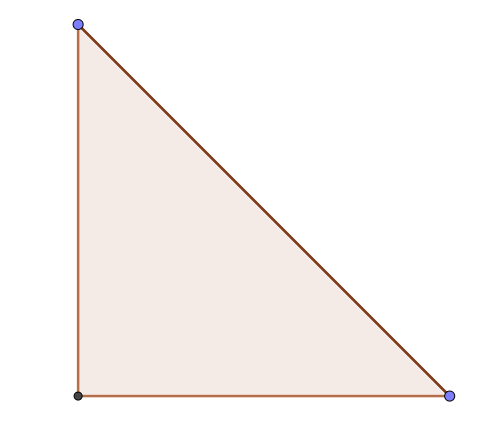
\includegraphics[width=0.7\textwidth]{Img1.PNG} % first figure itself
        \caption{Conjunto lineal puro}
    \end{minipage}\hfill
    \begin{minipage}{0.45\textwidth}
        \centering
        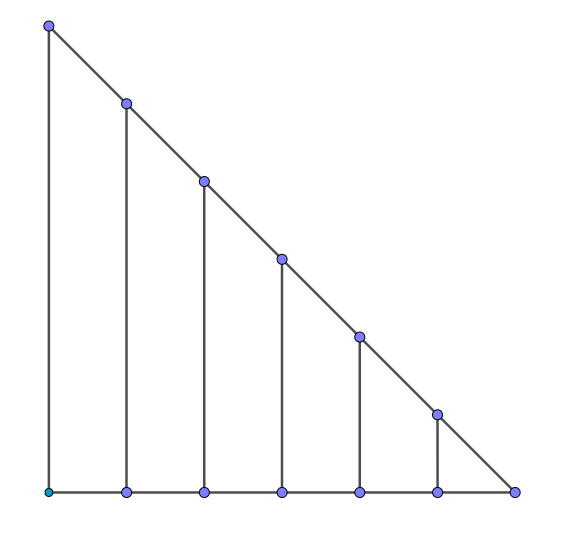
\includegraphics[width=0.65\textwidth]{Img2.PNG} % second figure itself
        \caption{Conjunto lineal mixto \newline \hspace*{1.5cm} Eje x variable entera \newline \hspace*{1.5cm} Eje y variable continua}
    \end{minipage}
    %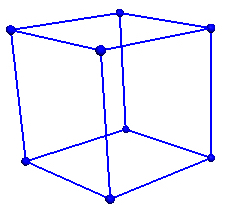
\includegraphics[width=0.3\textwidth]{cube3.jpg}
    %\caption{Conjunto lineal binario}
\end{figure}

\end{eje}
\newpage
\begin{figure}
    \centering
    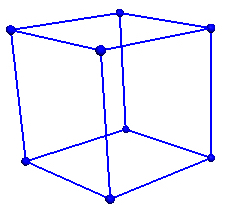
\includegraphics[width=0.3\textwidth]{cube3.jpg}
    \caption{Conjunto lineal binario}
\end{figure}
\begin{defi}[Programas lineales puros / mixtos / enteros / binarios] Diremos que un problema de la forma:
$$
\max\{c^{t}\colon x \in S\}
$$
es un \emph{programa lineal puro / mixto / entero / binario} si $S$ es un conjunto lineal puro / mixto / entero / binario. 
\end{defi}

Se abreviaran como \emph{PL / PLM / PLE / PLB} respectivamente.

\textbf{Observación:} A $S$ se le conoce como dominio o conjunto factible del programa.
\section{Modelos}

En general los problemas de optimización que aparecen en la vida real no están escritos como un PLM. Por ende es necesario reescribir un problema para poder trabajarlo como tal.

\begin{defi}[Modelo] Diremos que un PLM es modelo de un problema si

\begin{itemize}
    \item Cada solución óptima del PLM es solución óptima del problema original.
    \item Al menos una solución óptima del problema original es factible en el PLM
\end{itemize}
\end{defi}

Es importante notar que a veces se relaja la primera condición y se pide que sea algún tipo de solución óptima en particular. La definición anterior da la oportunidad de que existan soluciones óptimas del problema original que no sean factibles en el PLM, en caso contrario nos encontramos frente a un modelo particular:

\begin{defi}[Modelo exacto] Diremos que un PLM es un modelo exacto si las soluciones factibles del problema original están en correspondencia uno a uno, de manera explicita con las soluciones factibles del PLM
\end{defi}

\begin{eje}[Knapsack/ Problema de la mochila] Dado $n \in \NN$ objetos, valores $v_{i} \geq 0$ y tamaños $s_{i} \geq 0$. Dada una mochila de capacidad $B \geq 0$. Seleccionar un subconjunto a poner en la mochila maximizando el valor total.

\begin{equation*}
\begin{aligned}
\textrm{(Knapsack)}~ & \max
& & \displaystyle{\sum_{i \in [n]}}~v_{i}x_{i}\\
& \text{s.a.}
& & \displaystyle{\sum_{i \in [n]}}~s_{i}x_{i} \leq B\\
&&& x_{i} \in\{0,1\} ~ \forall i \in [n],
\end{aligned}
\end{equation*}
\newpage
donde
\begin{enumerate}
    \item $x_{i}=1 \iff i \text{  se encuentra en la mochila}$
    \item $\displaystyle{\sum_{i \in [n]}}~s_{i}x_{i}$ es la capacidad ocupada de la mochila.
    \item $\displaystyle{\sum_{i \in [n]}}~v_{i}x_{i}$ es el valor de la mochila.
\end{enumerate}

\end{eje}

\textbf{Observación 1:} Este modelo es exacto.

\textbf{Observación 2:} Es importante notar que a veces, por mucho que se conozcan técnicas para resolver un problema, es conveniente escribir el problema como un PLM, lo anterior permite la libertad de agregar restricciones fácilmente a los problemas de optimización.

\begin{eje}[s-t Camino de largo mínimo] Dado el digrafo $G=(V,\Vec{E})$, nodo de origen $s \in V$, nodo destino $t \in V$. Dada además una función de largos no negativos $\ell: \Vec{E} \to \RR_{+}$. Determinar un camino de largo mínimo de $s$ a $t$. Para resolver este problema, necesitamos caracterizar de alguna manera los $s$-$t$ caminos.  Veremos dos maneras de realizar esto:
\begin{enumerate}[\bf I.-]
    \item \textbf{(Mediante cortes)} Sea $x\in \{0,1\}^E$ en donde $\forall e\in E, ~x(e)=1 \iff$ el arco $e$ esta siendo ocupado.\\
    Recordemos la definición de corte:
    \begin{defi}[s-t corte] Un subconjunto $U \subseteq V$ es un $s$-$t$ corte si $s \in U, t \not \in U$. 
    \end{defi}
    Tambien recordemos las siguientes definiciones:
    \begin{defi}
    \hphantom{0.5 cm}
    \begin{itemize}
        \item $\delta^{+}(U)$ son los arcos que salen del conjunto $U$.
        \item $\delta^{-}(U)$ son los arcos que entran del conjunto $U$. 
    \end{itemize} 
    \end{defi}
    Para caracterizar que se sale de cada $U$ $s$-$t$ corte utilizaremos la siguiente ecuación:
    $$x(\delta^+(U)):= \sum\limits_{e\in \delta^+(U)} x(e) \geq 1 $$
    Así el problema lo podemos plantear como sigue:

\begin{equation*}
\begin{aligned}
\textrm{(SP-Conector)}~ & \min
& & \displaystyle{\sum_{e \in E}}~\ell_{e}x_{e}\\
& \text{s.a.}
& & x\left(\delta^{+}(U)\right) \geq 1 \text{ para todo }s\text{-}t \text{ corte } U \\
&&& x \in\{0,1\}^{E}
\end{aligned}
\end{equation*}


\begin{enumerate}
    \item Se puede probar que si el conjunto de arcos cruza todos los cortes entonces tiene que haber un $s$-$t$ camino.
    \item Hay $|\mathcal{P}(V\setminus\{s,t\})|=2^{n-2}$ cortes, y por ende $2^{n-2}$ restricciones.
\end{enumerate}
Se dejan los siguientes ejercicios propuestos:

\begin{ejer}
Probar que para el problema $s$-$t$ camino de coste mínimo y $\ell_e{} >0 ~ \forall e$ entonces SP-Conector es un modelo. Y probar que (en general) no es un modelo exacto.
\end{ejer}
\begin{ejer}
Modificar SP-Conector para que incluso cuando $\ell$ pueda tomar valores nulos sea un modelo.
\end{ejer}
\vspace{0.1 mm}
Es importante notar que la cantidad de restricciones crece de manera exponencial con el tamaño, luego, si bien el modelo soluciona el problema, en la practica el tiempo en que se ejecute el programa va a ser grande.

Por lo anterior es conveniente plantear el problema de otra manera. 
\NAM{}{\newpage}
    \item \textbf{(Mediante flujos)} Recordemos la definición de flujo: 
    
    
\begin{defi}[s-t flujo] Una función $f:E \to \RR_{+}$ es un $s$-$t$ flujo si:

$$
f\left(\delta^{+}(u)\right)=f\left(\delta^{-}(u)\right) ~ \forall u \in V \backslash\{t,s\}
$$
\end{defi}
Luego el problema es posible plantearlo como:

\begin{equation*}
\begin{aligned}
\textrm{(SP-Flujo)}~ & \min
& & \displaystyle{\sum_{e \in E}}~\ell_{e}x_{e}\\
& \text{s.a.}
& & x(\delta^{+}(u))=x(\delta^{-}(u))~ \forall u \in V \backslash\{t,s\} \\
&&& x(\delta^{+}(s))=x(\delta^{-}(t))=1\\
&&& x(\delta^{-}(s))=x(\delta^{+}(t))=0\\
&&& x \in\{0,1\}^{E}
\end{aligned}
\end{equation*}


De esta manera existen $n+2$ restricciones lo cual es una cantidad lineal de restricciones.

\begin{ejer}
Verifique que SP-Flujo es un modelo del problema cuando $\ell_{e} >0 ~\forall e$ y muestre que, en general, no es un modelo exacto.
\end{ejer}
\begin{ejer}
Modifique SP-Flujo para que sea un modelo incluso cuando $\ell$ pueda tomar valores nulos.
\end{ejer}

\begin{ejer}Pruebe que SP-Flujo es equivalente a

\begin{equation*}
\begin{aligned}
& \min
& & \displaystyle{\sum_{e \in E}}~\ell_{e}x_{e}\\
& \text{s.a.}
& & x(\delta^{+}(u))=x(\delta^{-}(u))~ \forall u \in V \backslash\{t,s\} \\
&&& x(\delta^{+}(s))-x(\delta^{-}(s))=1\\
&&& x \in\{0,1\}^{E}
\end{aligned}
\end{equation*}


\end{ejer}
    
\end{enumerate}

Mostraremos en el curso que el problema es posible relajarse y en vez de considerar $x\in \{0,1\}^{E}$ se puede transformar al problema lineal puro con la restricción  $0 \leq x \leq 1$.




\end{eje}


% \end{document}

%%%%%%%%%%%%%%%%%%%%%%%%%%%%%%%%%%%%%%%%%%%%%%%%%%%%%%%%%%%%%%%%%%%%%%%%%%%%%%%%%%%%%%%%%%%%
%%%%%%%%%%%%%%%%%%%%%%%%%%%%%%%%%%%%%%%%%%%%%%%%%%%%%%%%%%%%%%%%%%%%%%%%%%%%%%%%%%%%%%%%%%%%
%!TEX root = ../notas_de_clase.tex

%%%%% NOMBRE ESCRIBAS Y FECHA
\renewcommand{\sca}{Matías Azócar}
\renewcommand{\scb}{Carolina Chiu}
\renewcommand{\scc}{Francisco Muñoz}
\renewcommand{\catnum}{2} %numero de catedra
\renewcommand{\fecha}{23 de marzo de 2020}

%%%%%%%%%%%%%%%%%%

% \begin{document}
%Encabezado

% notas al margen
% \ifnum \notasalmargen=1
% \newgeometry{left=1.5cm,top=1.5cm,right=1.5cm, bottom=1.5cm,letterpaper, includeheadfoot, outer=5cm, heightrounded, marginparwidth=4cm, marginparsep=-2.5cm}
% \fi
\NAM{
\newgeometry{left=1.5cm,top=1.5cm,right=1.5cm, bottom=1.5cm,letterpaper, includeheadfoot, outer=5cm, heightrounded, marginparwidth=4cm, marginparsep=-2.5cm}
\savegeometry{notas-al-margen}
}{}

%fin de notas al margen

\fancyhead[L]{Facultad de Ciencias Físicas y Matemáticas}
\fancyhead[R]{Universidad de Chile}
\vspace*{-1.2 cm}
\NAM{\begin{minipage}{0.7\textwidth}}{0.6\textwidth}
\begin{flushleft}
\hspace*{-0.5cm}\textbf{MA4702. Programación Lineal Mixta. 2020.}\\
\hspace*{-0.5cm}\textbf{Profesor:} José Soto\\
\hspace*{-0.5cm}\textbf{Escriba(s):} \sca, \scb ~y \scc.\\
\hspace*{-0.5cm}\textbf{Fecha:} \fecha.
\end{flushleft}
\end{minipage}
\NAM{\begin{minipage}{0.4\textwidth}}{\begin{minipage}{0.36\textwidth}}
\begin{flushright}
\NAM{\hspace*{4.3cm}
\includegraphics[scale=0.15]{fcfm}}{
\includegraphics[scale=0.15]{fcfm}}
\end{flushright}
\end{minipage}
\bigskip

\begin{center}
\LARGE\textbf{Cátedra \catnum}
\end{center}

%Fin encabezado

\section*{Introducción}

En esta cátedra se verán dos temas principales: se comenzará dando un recorrido por la historia de los algoritmos PL/PLM a modo de motivación, para después retomar el contenido de la clase pasada y estudiar más en detalle el concepto de las \textit{formulaciones}.

\section{Historia de Algoritmos PL/PLM}
¿Por qué utilizamos algoritmos de PL/PLM sobre programación no lineal o convexa? Algunas razones son:
\begin{itemize}
    \item Permiten modelar una gran variedad de problemas de la vida real con suficiente generalidad.
    \item Existen buenos algoritmos (a nivel práctico y teórico) y heurísticas\footnote{Una \textbf{heurística} es una técnica diseñada para resolver un problema más rápidamente cuando los métodos clásicos son demasiados lentos, o bien, encontrar una solución cercana al óptimo cuando los métodos clásicos fallan.} que permiten solucionarlas.
    \item Han tenido éxito industrial (existen solvers bien implementados).
\end{itemize}

\subsection*{Orígenes de la Programación Lineal Pura}
\begin{itemize}
    \item \textbf{1827 y 1836}: \textit{Fourier} y \textit{Motzkin} (por separado) describen un método \textbf{finito} para sistemas de desigualdades (conocido como \textit{esquema de eliminación de Fourier-Motzkin}).
    \item \textbf{1937}:\textit{Kantorovich} (Premio Nobel 1975) desarrolla una teoría de dualidad en programación lineal para temas de economía. 
    \item \textbf{1946}: \textit{George Dantzig} desarrolló la base del método Simplex mientras trabajaba para la fuerza aérea de Estados Unidos. Por otro lado, \textit{Jon Von Neumann} desarrolla la teoría de la dualidad en programación lineal.  Ambos junto a Kantorovich se consideran los padres de la programación lineal.
\end{itemize}
%Aquí falta q Simplex no es polinomial y la pregunta de si los PL lo son, etc

\begin{defi}[Algoritmo Polinomial]
Se define como \textit{algoritmo polinomial} a un algoritmo con entrada de $N$ bits, y que ejecuta sus instrucciones en un orden de \Ord[p(N)], donde $p$ es un polinomio. Es decir, un algoritmo con tiempo de ejecución $N^{\Ord[1]}$.
\end{defi}
\begin{defi}[Algoritmo Exponencial]
Se define como \textit{{algoritmo exponencial}} a un algoritmo con entrada de $N$ bits, y que ejecuta sus instrucciones en un orden de \Ord[e^{N}]. Es decir, por ejemplo, un algoritmo al cual le toma $2^{\Ord[N]}$ operaciones en ejecutarse.
\end{defi}
\begin{eje}
Un algoritmo que se tome como máximo $N^{50}$ operaciones en ejecutarse, es un algoritmo polinomial\footnote{Aunque no uno muy eficiente.}.
\end{eje}
\begin{eje}
El algoritmo de Kruskal es polinomial.
\end{eje}
La gran ventaja de este tipo de algoritmos es que si el tamaño de la instancia crece, por ejemplo, se duplica, entonces el tiempo de ejecución sólo se multiplica por una constante. Por ejemplo, un algoritmo con cota $N^k$ en su tiempo de ejecución, al ser alimentado por una instancia de tamaño $2N$, su tiempo cambia a $(2N)^{k}=2^k N^k$.

En cambio, si se está trabajando con un algoritmo exponencial, al duplicar el tamaño de la instancia, la complejidad del algoritmo podría crecer demasiado. Por ejemplo, para un algoritmo con cota $2^{cN}$ en su tiempo de ejecución, la cota para una instancia de tamaño $2N$ se eleva al cuadrado (pues $2^{2cN}=(2^{cN})^2$).

\begin{defi}[Clase P]
La \textit{{clase P}} contiene a aquellos problemas que son solubles en tiempo polinómico.
\end{defi}
\begin{eje}
El problema de calcular un matching es de clase P, pues existe una solución en tiempo polinomial.
\end{eje}

Existe una clase de problemas, llamados NP-completos (cuya definición formal no daremos en este curso) que ocurren muchas veces en la práctica. Se conjetura (no ha sido demostrado) que todos estos problemas no están en P.

\begin{obs}
La pregunta ¿$P=NP$? es aún un problema abierto y es uno de los problemas del milenio\footnote{Es decir, si es que alguien demuestra o refuta la conjetura, ¡se ganará un millón de dolares!.}.
\end{obs}

Se han definido estos conceptos de complejidad para responder a la siguiente pregunta: ¿Qué clase de problema es PL? la pregunta tiene su importancia, pues Klee y Minty (1973) demostraron que Simplex \textbf{no es polinomial}\footnote{Más precisamente, demostraron que hay instancias para los cuales Simplex debe tomar un número superpolinomial de pasos}, a pesar de que es muy rápido en la mayoría de las instancias.

Entonces, ¿Es PL demasiado general como para no estar en P? La respuesta es: ¡No!, en efecto en el año 1979 se demuestra que \textbf{PL está en P}.

\subsection*{Programación Lineal Pura hoy en día}
Ha sido trabajo de los matemáticos el de reducir el tiempo de ejecución del PL. En lo que sigue, $n$ corresponde a variables y $L$ al número de bits que se usan para codificar la entrada.
\begin{itemize}
    \item \textbf{1979}: \textit{Khachiyan} desarrolla el método de la elipsoide para PL (Complejidad $\Ord[n^6L]$).
    \item \textbf{1984}: \textit{Karmakar} desarrolla el método de punto interior (Barrera) para PL (Complejidad $\Ord[n^{3,5}L]$).
    \item \textbf{2015}: \textit{Lee y Sidford} desarrollan la primera mejora en 20 años para flujo en redes (Complejidad $\Ord[n^{2,5}L]$).
    \item \textbf{2019}: \textit{Cohen, Lee y Song} obtienen una complejidad de $\Ord[n^{2,37}L]$ usando multiplicación rápida de matrices.
\end{itemize}

\begin{obs}
Notar que una complejidad de \Ord[n^6 L] es bastante alta, pero al menos es polinomial. Por otro lado, \Ord[n^{2,37} L] ya es una complejidad cercana a una cuadrática, el cuál es un orden más aceptable.
\end{obs}

\begin{obs}
En la práctica, ninguno de estos algoritmos se utiliza (ya que son muy difíciles de implementar, y algunos resultan peores que un algoritmo exponencial en regímenes pequeños). Lo que se usa son mezclas de Simplex, Simplex-dual y Barrera.
\end{obs}

Respondiendo a la pregunta de por qué se prefiere PL/PLM, es porque hoy en día tenemos muchos métodos de resolución a estos problemas. De forma que, se ha avanzado tanto en esta área, que programas lineales que antes tomaban 20 años de procesar, hoy en día se pueden resolver en un segundo. Esto permite utilizar millones de variables y restricciones y resolverlos en un tiempo prudente.

\subsection*{¿Qué pasa con PLE y PLM?}
\begin{itemize}
    \item En la década de 1960 sale el primer solver comercial.
    \item Las siguientes décadas se dedican a crear mejoras en la implementación de PL.
    \item En la década de 1990 aparecen solvers nuevos, como \textit{CPLEX} (ILOG), \textit{MINTO} (Gerogia Tech) y \textit{XpressMP} (comercial).
    \item En el año 2007 IBM compra ILOG.
    \item Los creadores originales de \textit{CPLEX} no se involucran con IBM, y en su lugar fundan \textit{Gurobi} en el año 2009.
\end{itemize}

Hoy en día, los problemas de programación lineal entera se pueden resolver de forma rápida debido a que se han incorporado una serie de ideas (que se verán más adelante en el curso) a los solvers previamente mencionados. Algunas de ellas son:
\begin{itemize}
    \item Aproximación sucesiva de PLE por PL.
    \item Agregar planos cortantes, es decir, incluir restricciones sin perder puntos factibles (mejora en la formulación).
    \item \textit{Branch and Bound}: es la base de los algoritmos PLE. La idea es que si hay un conjunto finito de puntos que pueden ser solución, se pueden enumerar de manera sistemática (como árbol) y es posible darse cuenta que hay ramas del árbol que no pueden ser solución.
    \item Planos cortantes genéricos: cortes que se generan automáticamente (Gomory, MIR, etc.)
    \item Presolver (Técnicas de reducción de tamaño).
    \item Generación de filas y columnas; Simetría; Heurísticas; entre otras.
\end{itemize}

Probablemente PLE no está en P (se puede probar que es NP-Completo). Sin embargo, los solvers disponibles actualmente son capaces de:
\begin{itemize}
    \item Realizar buenas aproximaciones de soluciones de PLE con millones de variables y restricciones. Estas soluciones son factibles y pueden reportar que se encuentran cerca del óptimo. (para hacer esto, no se necesita que el usuario sea un experto, sólo basta con saber ocupar dichos solvers).
    \item Resolver a optimalidad muchas clases de subproblemas.
    \item Todo eso se hace prácticamente sin intervención del usuario.
\end{itemize}

\section{Formulaciones}
\begin{defi}[Poliedro] Un \emph{poliedro} $P$ es un conjunto lineal puro, es decir
$$P=P(A,b)=\{x\in \RR^n:Ax\leq b\}$$
con $A\subseteq \RR^{n\times m}$ y $b\in \RR^n$
\end{defi}
\begin{itemize}
    \item Si $A$ y $b$ pueden ser escogidos racionales (es decir, sus componentes pueden ser escogidas racionales): $P$ es un \textbf{poliedro racional}.
    \item Si $P$ es acortado: se llama \textbf{polítopo}.
\end{itemize}
\begin{obs}
Dado que los poliedros son intersecciones finitas de semiplanos, y los semiplanos son conjuntos convexos, entonces los poliedros son \textit{conjuntos convexos}.
\end{obs}
\begin{defi}[Formulación] Un poliedro $P$ es una \emph{formulación} para un conjunto $S\subseteq\ZZ^E \times \RR^ C$ si:
$$S=P\cap (\ZZ^E \times \RR^C)$$
\end{defi}
En otras palabras, una formulación es un poliedro que aproxima externamente bien a algún conjunto.

\begin{eje} \label{eje:formulacion1}
En la Figura \ref{fig:formulacion1}, se puede observar un poliedro $P$ (conjunto verde) que es una formulación de un conjunto $S$ (puntos rojos), pues $$S = P \cap \ZZ^{E}$$ 
\begin{figure}[H] 
    \centering
    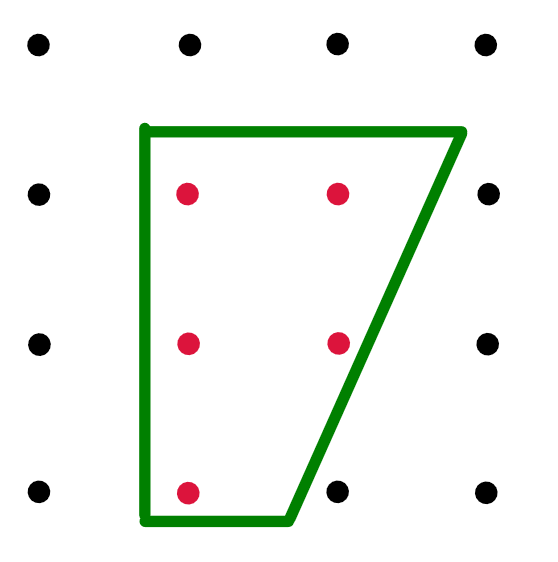
\includegraphics[scale=0.3]{formulacion1.png}
    \caption{Primer ejemplo de una formulación.}
    \label{fig:formulacion1}
\end{figure}
\end{eje}

Podemos notar que las formulaciones no son necesariamente únicas, en efecto, en el Ejemplo \ref{eje:formulacion1} se puede encontrar otro poliedro $P'$, tal como se presenta en el siguiente ejemplo:

\begin{eje} \label{eje:formulacion2}
En la imagen \ref{fig:formulacion2}, se puede observar un poliedro $P'$ (conjunto azul) que es una formulación de un conjunto $S$ (puntos rojos), pues $$S = P' \cap \ZZ^{E}$$ 
\begin{figure}[H] 
    \centering
    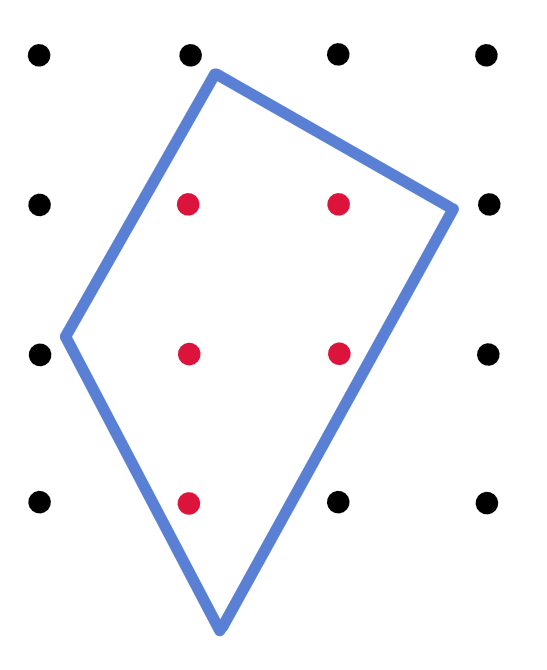
\includegraphics[scale=0.3]{formulacion2.png}
    \caption{Segundo ejemplo de una formulación.}
    \label{fig:formulacion2}
\end{figure}
\end{eje}

Dicho esto, nos podemos preguntar: ¿Cuál de todas las formulaciones ocupar? La respuesta que nace naturalmente es: ocupar la formulación minimal para $S$. Esto se puede lograr ocupando como formulación para $S$ su envoltura convexa, vale decir, $\conv S$. Una representación de lo anteriormente dicho se puede observar en la siguiente figura:

\begin{figure}[H] 
    \centering
    
\includegraphics[scale=0.3]{formulacion3.png}
    \caption{Formulación minimal para $S$: su envoltura convexa.}
    \label{fig:formulacion3}
\end{figure}


Formalizando lo comentado anteriormente en los ejemplos, $P$ es buena formulación de $S$ si es que lo \emph{aproxima} apropiadamente. Para empezar, al menos, sabemos que debemos tener lo siguiente 
\begin{center}
$S\subseteq P$
\end{center}
\begin{itemize}

    \item Sean $P_1\subseteq P_2$ dos formulaciones para el mismo conjunto. En este contexto, diremos que $P_1$ es \emph{mejor} que $P_2$.
    
    Posterior a esto, no es difícil pensar que el mejor de todos los casos será tomar como formulación la envoltura convexa (esto puede, y debería, ser demostrado). Justamente por eso tenemos lo siguiente
    
    \item Si $P=\conv(S)$ entonces $P$ es \emph{formulación ideal} de $S$.
\end{itemize}

\begin{obs}No todos los conjuntos lineales mixtos admiten formulaciones ideales. \end{obs}

En la siguiente figura se puede apreciar un ejemplo de lo anterior, pues, para la primera restricción (gráficamente, la diagonal) no hay valores que se alcancen en la frontera. Esto, pues habría que solucionar $-\sqrt2 x+y=0$ con $x,\ y$ enteros. Sin embargo, por la irracionalidad de $\sqrt2$ no habrá un punto $(x,y)$ que resuelva tal ecuación. Lo que sucederá es que iremos tomando una cantidad infinita de puntos que se acerquen, pero eso no define un poliedro. Así, se evidencia que hay conjuntos que no admiten formulación ideal. 
\begin{figure}[H]
    \centering
    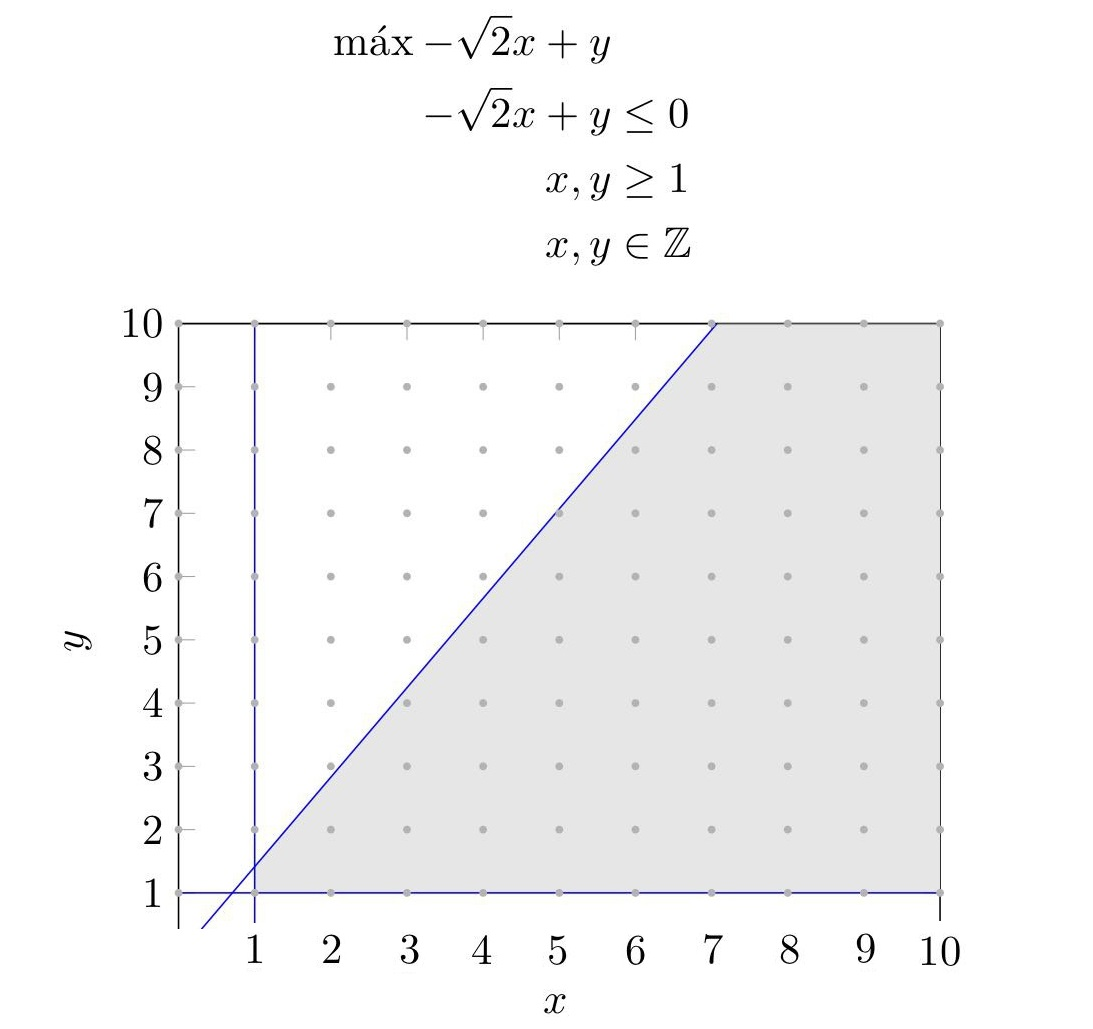
\includegraphics[scale=0.18]{Imagen1.jpg}
    \caption{Ejemplo de PLM donde no existe formulación ideal.}
    \label{fig:NoExistenceIdeal}
\end{figure}

Notemos que lo anterior no sucede para un PL puro, recordando del curso de optimización, que todo PL factible y con objetivo acotado alcanza su óptimo.

\begin{teo}
Sea (\textit{M}) un PLM con datos racionales. Si su relajación lineal (\textit{P}) es acotado en la dirección de optimización, entonces o bien (\textit{M}) tiene óptimo finito racional y alcanzable, o bien (\textit{M}) es infactible.
\end{teo}

\begin{eje}[Uncapacitated Facility Location] Un problema clásico en Investigación de Operaciones es el de \emph{Uncapacitated Facility Location}. Definimos ahora lo que se recibe como información y lo que busca hallar el problema.

\begin{figure}[H]
    \centering
    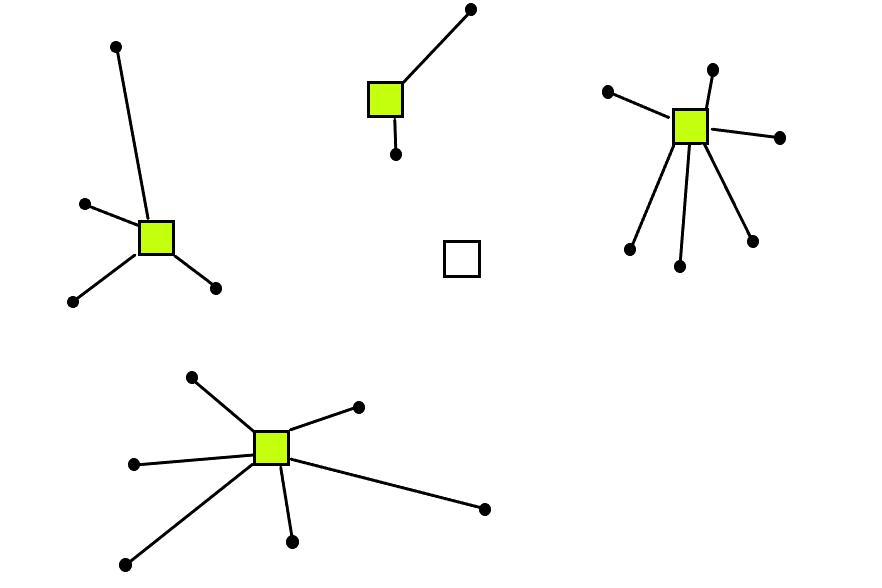
\includegraphics[scale=0.25]{UFL.png}
    \caption{Visualización del problema \textit{Uncapacitated Facility Location}.}
    \label{fig:UFL}
\end{figure}

\textbf{Entrada:} $n$ clientes y $m$ ubicaciones de bodegas. Existe un costo fijo $c_j\geq 0,\ \forall j\in [m]$ asociado a la apertura de una bodega y un costo de conexión $d_{ij}\geq 0$ por conectar a un cliente $i$ con una bodega $j$, $\forall i\in[n]$, $\forall j\in[m]$.

\textbf{Objetivo:} Abrir bodegas y conectar clientes a bodegas abiertas incurriendo en un costo total mínimo.

Construiremos una formulación para el problema:

Para ello haremos uso de dos variables binarias:
$$y_j=\begin{cases}1\text{ si la bodega }j\text{ abre.}\\
0\text{ si no lo hace}\end{cases}\hspace{0.5cm}x_{ij}=\begin{cases}1\text{ si el cliente } i\text{ conecta con la bodega }j\\
0\text{ si no lo hace}
\end{cases}$$
De esta forma, procederemos a plantear la formulación. Queremos minimizar el costo total, así, el objetivo será:
$$\text{(FL1)}\hspace{0.5cm}\min \sum_{j\in[m]}c_j y_j + \sum_{i\in [n]}\sum_{j\in[m]}x_{ij}d_{ij}$$
El primer término será el asociado a los costos fijos de las bodegas y el de la derecha el costo de conexión cliente-bodega total.

Ahora, las restricciones serán las siguientes:

\begin{equation*}
    \begin{array}{rll}
        s.a.&\sum\limits_{j\in[m]}x_{ij}=1&\forall i \in [n]\\
        &\sum\limits_{i\in [n]}x_{ij}\leq n\cdot y_j&\forall j \in [m]\\
        &x_{ij},\ y_{j}\in\{0,1\}&\forall i\in[n]\text{ }\forall j\in[m]
    \end{array}
\end{equation*}

La primera restricción es la que indica que de todas las bodegas, el cliente \emph{debe} estar asociado a una. (Podría ser reemplazado por la restricción de estar asociado al menos con una). La segunda viene de la siguiente situación:
\begin{itemize}
    \item Si la bodega no abre ($y_j=0$) no pueden haber clientes asociados a esa bodega, luego, como los $x_{ij}$ son no negativos, deben ser todos cero.
    \item Si la bodega abre ($y_j=1$) entonces pueden haber como máximo $n$ clientes asociados a esa bodega (pues ese es el número total de clientes)
\end{itemize}
La tercera restricción viene del hecho de que definimos $x_{ij}$ y $y_j$ como variables binarias. 

El objetivo junto a las tres restricciones definen la formulación que hemos construido.
\end{eje}


\begin{eje}[Problema de Asignación] Un problema al que probablemente usted ha podido enfrentarse en Algoritmos Combinatoriales es el \emph{problema de asignación.}

\begin{figure}[thb]
\centering
\begin{tikzpicture}[scale=1]
    %Origen
    \node[draw,circle] (p1) [label=above:Personas]   at (0,5) {1};
    \node[draw,circle] (p2) []                       at (0,4) {2};
    \node              ()                                            at (0,3) {$\vdots$};
    \node[draw,circle] (pi) []                       at (0,2) {$i$};
    \node              ()                                            at (0,1) {$\vdots$};
    \node[draw,circle] (pn) []                       at (0,0) {$n$};
    %Destino
    \node[draw,circle] (t1) [label=above:Tareas] at (7,5) {1};
    \node[draw,circle] (t2) []                      at (7,4) {2};
    \node              ()                                            at (7,3) {$\vdots$};
    \node[draw,circle] (tj) []                      at (7,2) {$j$};
    \node              ()                                            at (7,1) {$\vdots$};
    \node[draw,circle] (tn) []                      at (7,0) {$n$};
    \draw[->, dashed] (p1) -- (t2);
    \draw[->, dashed] (p2) -- (tn);
    \draw[->, dashed] (pi) -- (t1);
    \draw[->, dashed] (pn) -- (tj);    
\end{tikzpicture}
\caption{Problema de Asignacion.}
\label{fig:prob_asign}
\end{figure}

\textbf{Entrada:} $n$ tareas y $n$ personas. Cada persona debe realizar \emph{exactamente} una tarea. $c_{ij}$ es el costo incurrido por la persona $i$ al realizar la tarea $j$.

\textbf{Objetivo:} Encontrar la asignación de costo total mínimo.



Construiremos una formulación para el problema:

Para ello haremos uso de una variables binaria:
$$x_{ij}=\begin{cases}1\text{ si la persona } i\text{ realiza la tarea }j\\
0\text{ si no lo hace}
\end{cases}$$
Así, procedemos. Queremos minimizar el costo total, así, el objetivo será:
$$\text{(}A\text{)}\hspace{0.5cm} \min \sum_{i\in[n]}\sum_{j\in [n]}c_{ij} x_{ij}$$
El término proviene de sumar los costos de las personas (suma sobre $i$) asociadas a las tareas (suma sobre $j$), los cuales contaremos solo si la persona $i$ realiza la tarea $j$.

Ahora, las restricciones serán las siguientes:

\begin{equation*}
    \begin{array}{rll}
        s.a.&\sum\limits_{j\in[n]}x_{ij}=1&\forall i \in [n]\\
        &\sum\limits_{i\in [n]}x_{ij}=1&\forall j \in [n]\\
        &x_{ij},\in\{0,1\}&\forall i\in[n]\text{ }\forall j\in[n]
    \end{array}
\end{equation*}
El objetivo junto a las tres restricciones definen la formulación que hemos construido. \\

Ahora, definiremos lo siguiente:
\begin{itemize}
    \item $S$: Dominio de ($A$)
    \item $D$: Relajación de ($A$)
\end{itemize}


Gracias a un importante resultado de Birkhoff y Von Neumann sabemos que todo punto en $P$ es combinación convexa de puntos enteros (en $S$), Luego, $P$ es ideal.
\end{eje}

Para finalizar la clase, se presenta un caso interesante. \\
Sea ($M$) un PLE (totalmente) acotado, con dominio $S$. Luego $S$ es finito. ¿Tiene formulación ideal?
\begin{align*}
    S &=\{s_i\}_{i=1}^K\\
    \conv(S) &=\{x=\sum_{i=1}^K \lambda_i s_i:\lambda_i\geq 0,\ \sum_{i=1}^K \lambda_i=1\}
\end{align*}
Surge así la pregunta\ldots
¿La envoltura convexa de un conjunto finito de puntos es un poliedro? (esto puede ser respondido a través del estudio de teoría poliedral).


\begin{comment}
En la red hay bastante material para aprender a usar esta herramienta. Como ejemplo, les recomiendo visitar
\url{http://latex-project.org/guides/} y \url{http://texblog.net/}.

Además, es bueno empezar a seguir buenas prácticas, dejando de lado un montón de comandos que están obsoletos (en particular, reemplazar \verb+\eqnarray+ y \verb+$$ ... $$+ por los más modernos \verb+\align+ y \verb+\[ ... \]+).

\subsection{Recomendaciones para escribir un apunte}
Es bueno comenzar cada clase con una frase introductoria, explicando lo que se va a ver. No llegue y copie textualmente lo que se ve en la pizarra / video sin incorporar comentarios que aclaren (en clases, suelo decir mucho más de lo que escribo).

Recuerde que las ecuaciones también son parte del texto, y luego deben cumplir las reglas de puntuación (por ejemplo, usar comas y puntos
finales).

\subsection{Algunos ejemplos}

\subsubsection*{Uso simple de macros:}
\begin{defi}[Cintura de un grafo]
 La \emph{cintura} de un grafo es el largo del ciclo más corto. Si el grafo es acíclico, se define como $+\infty$.
Denotaremos la cintura de $G$ por $\cin(G)\in \ZZ$. 
\end{defi}
Observar (en la fuente) la definici\'on de las macros \verb+\Z+ y \verb+\cin+.

\begin{lem}
 Si $G$ es un grafo bipartito entonces $\cin(G)\ge 3$.
\end{lem}

M\'as ejemplos: Escriba $\min(X)$ (\begin{verb}$\min(X)$\end{verb}) en vez de $min(X)$ (el \'ultimo parece producto de $m$, $i$ y $n$). 
Por lo mismo, escriba tambi\'en $X_{\text{opt}}$ (\begin{verb}$X_{\text{opt}}$\end{verb}) en vez de $X_{opt}$.


\subsubsection*{Ecuaciones alineadas.}

No es difícil escribir ecuaciones que tengan una sola alineación como
\begin{align}
\psi(n)
&= \frac{(2n)!}{n! 2^n} = \frac{(2n)(2n-1) \dotsm (n+1)}{2^n} \notag \\
&\geq \left( \frac{n}{2} \right)^n. \label{eqn:interesante}
\end{align}

Sin embargo, escribir un PL en \LaTeX{} puede ser complicado. Un formato tipo para escribir simultáneamente un primal y un dual es el siguiente:

\begin{alignat*}{5}
&\max\        & \sum_{ij \in E} x_{ij}w_{ij} &		 &                      &\qquad\qquad \min\        &\sum_{i \in V}y_i&\\
&\text{s.a. } & \sum_{j\colon j\neq i} x_{ij}&\leq 1 &\quad\forall i \in V  &\qquad\qquad \text{s.a. } &y_i+y_j &\geq w_{ij} &\quad\forall ij \in E\\
&	          & x_{ij}                       &\geq 0 &\quad\forall ij \in E &\qquad\quad               &y_i &\geq 0      &\quad\forall i \in V.
\end{alignat*}

\medskip
Este es solo un documento de ejemplo. Entre otras cosas \LaTeX{} permite escribir fácilmente
\begin{itemize}
  \item Matrices.
  \item Integrales.
  \item Tablas.
  \item Listas.
  \item etc.
\end{itemize}
 
\subsection{Ejemplo}

Como ejemplo adjunto el principio de la primera cátedra a continuación.

\begin{defi}[Problema de optimización e instancias] Un \textit{problema de optimización} $\mathcal{P}$ es un conjunto de \textit{instancias}. Cada \textit{instancia} está definida por:
\begin{itemize}
\item Un conjunto factible $S$.
\item Una función a optimizar $f: S \to \RR$.
\item Un objetivo, minimizar o maximizar la función $f$ en dicho conjunto $S$.
\end{itemize}
\end{defi}

Usualmente las instancias se describen de manera implícita o compacta.  Por ejemplo:

\begin{eje}[Árbol cubridor de peso mínimo -- minimum spanning tree, MST]
Cada instancia del problema (MST) se describe de manera compacta indicando un grafo $G=(V,E)$ con pesos en las aristas $w\colon E \to \RR_+$. De estos datos uno puede deducir el conjunto $S$ de todos los árboles cubridores de $G$, y para cada árbol $T\in \mathcal{S}$, el valor de la función es la suma de los pesos de las aristas $w(T)=\sum_{e\in T}w(e)$. El objetivo es minimizar la función de peso $w$.
\end{eje}
\end{comment}
%%NO ESTA LISTO TENGO Q TERMINAR EL ULTIMO EJEMPLO UWU

% \end{document}

%%%%%%%%%%%%%%%%%%%%%%%%%%%%%%%%%%%%%%%%%%%%%%%%%%%%%%%%%%%%%%%%%%%%%%%%%%%%%%%%%%%%%%%%%%%%
%%%%%%%%%%%%%%%%%%%%%%%%%%%%%%%%%%%%%%%%%%%%%%%%%%%%%%%%%%%%%%%%%%%%%%%%%%%%%%%%%%%%%%%%%%%%


%!TEX root = ../notas_de_clase.tex

%%%%% NOMBRE ESCRIBAS Y FECHA
% \rerenewcommand{\sca}{Escriba Uno}
% \rerenewcommand{\scb}{Escriba Dos}
% \rerenewcommand{\scc}{Escriba Tres}
\renewcommand{\catnum}{3} %numero de catedra
\renewcommand{\fecha}{27 de Marzo 2020}

%%%%%%%%%%%%%%%%%%

% \begin{document}
\shorthandoff{>}\shorthandoff{<}
%Encabezado

% notas al margen
\NAM{
\newgeometry{left=1.5cm,top=1.5cm,right=1.5cm, bottom=1.5cm,letterpaper, includeheadfoot, outer=5cm, heightrounded, marginparwidth=4cm, marginparsep=-2.5cm}
\savegeometry{notas-al-margen}
}{}
%fin de notas al margen

\fancyhead[L]{Facultad de Ciencias Físicas y Matemáticas}
\fancyhead[R]{Universidad de Chile}
\vspace*{-1.2 cm}
% notas al margen
\NAM{\begin{minipage}{0.7\textwidth}}{\begin{minipage}{0.6\textwidth}}
\begin{flushleft}
\hspace*{-0.5cm}\textbf{MA4702. Programación Lineal Mixta. 2020.}\\
\hspace*{-0.5cm}\textbf{Profesor:} José Soto\\
% \hspace*{-0.5cm}\textbf{Escriba(s):} \sca, \scb ~y \scc.\\
\hspace*{-0.5cm}\textbf{Fecha:} \fecha.
\end{flushleft}
\end{minipage}
% notas al margen
\NAM{\begin{minipage}{0.4\textwidth}}{\begin{minipage}{0.36\textwidth}}
\begin{flushright}
% notas al margen
\NAM{\hspace*{4.3cm}
\includegraphics[scale=0.15]{fcfm}}{
\includegraphics[scale=0.15]{fcfm}}
\end{flushright}
\end{minipage}
\bigskip

\begin{center}
\LARGE\textbf{Cátedra \catnum}
\end{center}

%Fin encabezado

\section{Descripción de Branch and Bound}

Uno de los métodos más usados para resolver PLM y otros problemas de optimización es \textbf{branch and bound (BnB)}. Se basa en la siguiente idea: 

\begin{quote}
Sea $\{S_1,\dots, S_k\}$ una partición del conjunto factible $S$ de un problema de optimización $z^*=\max \{c^Tx\colon x\in S\}$.
    Si $z^*_i=\max\{c^Tx\colon x\in S_i\}$ entonces $z^*=\max_{i\in [k]}z^*_i.$
\end{quote}

    BnB consiste en particionar el conjunto factible $S$ del problema original en conjuntos más pequeños y resolver luego $\max c^Tx$ en cada subconjunto de manera recursiva. Si la recursión se pudiera llevar completamente, al final  enumeraríamos todos los puntos factibles del problema. Esta idea tiene dos problemas. Primero, si el dominio es infinito entonces esto no es posible. Segundo, incluso si el dominio es finito, esto podría ser extremadamente lento y no difiere en nada de simplemente de simple fuerza bruta. 

    La idea es que BnB no explore todo el árbol de recursión sino que guarde cotas para los subproblemas que ya ha resuelto y, usando estas cotas determinar que no necesitamos resolver ciertos subproblemas. 
    
    En lo que sigue nos enfocaremos en PLM de la forma    
$$\begin{aligned}
    \qquad (M)&\quad \max c^Tx \\
    S&\colon \begin{cases}
    Ax &\leq b\\
    x &\in \ZZ^E\times \RR^C
    \end{cases}\quad
    \end{aligned}$$\\[5pt]
    donde $A$, $b$, $c$ son racionales. Llamemos $P=\{x\in \RR^{E\times C}, Ax\leq b\}$ a la relajación lineal natural de $S$, luego $S \subseteq P.$  Como los datos son racionales tenemos que el programa lineal relajado 
    \NAM{
    $$\begin{aligned}
        \qquad (L)&\quad \max c^Tx\\
        P&\colon \begin{cases}
        Ax &\leq b\\
        x&\in \RR^{E\cup C}
        \end{cases}\quad
        \end{aligned}$$\\[-20pt]
    }{
    $\begin{aligned}
        \qquad (L)&\quad \max c^Tx\\
        P&\colon \begin{cases}
        Ax &\leq b\\
        x&\in \RR^{E\cup C}
        \end{cases}\quad
        \end{aligned}$\\[5pt]
    }
        
    es o bien \textbf{infactible}, o bien \textbf{factible no acotado} o bien \textbf{factible acotado} con solución óptima $\bar{x}\in P$ racional. En este caso llamamos $\bar{z}=c^T\bar{x}$ a su valor.
    
    Llamemos $(M_0)$ al problema inicial dado y \textbf{pediremos que $(P_0)$ sea factible acotado}. Hacemos esto pues  BnB \emph{a secas} no es capaz de lidiar con problemas con relajación no acotada en la dirección de optimización.
    
    
    
    
    
    
    
    Para resolver $(M_0)$ se construye \textbf{iterativamente} un árbol $\calT$ cuyos nodos son de la forma $(M,B,s)$ con $(M)$ un subproblema de $(M_0)$, $B$ una cota superior (optimista) del valor de $(M_0)$, y $s$ un \textbf{status} que puede ser \textbf{activo}, \textbf{ramificado}, \textbf{infactible}, \textbf{dominado} o \textbf{entero}. Tanto la cota como el status de un nodo puede cambiar a lo largo del algoritmo.
    
    En el árbol  siempre se tendrá que \textbf{la unión de los dominios de las hojas} es el \textbf{dominio} de la raíz. Además se mantiene globalmente una solución factible (inicialmente nula) $x^*$ llamada \textbf{incumbente} que resulta ser la mejor solución encontrada hasta ahora y $z^*=c^Tx^*$ su valor (también llamada \textbf{mejor cota inferior}).
    Inicialmente, el nodo raíz es $(M_0,B_0,\text{activo})$ donde $M_0$ es el PLM original y $B_0$ es el valor $\bar{z}$ de su relajación. Además, $x^*$ es nulo y $z^*=-\infty$. Durante el algoritmo BnB hay 2 procesos importantes: la \textbf{creación de un nodo} y la \textbf{ramificación de un nodo activo}.
    
    
    %Abajo describimos la creación de un nodo $(M)$ y como se determina sus cotas y status.
    
    \begin{algorithm}[H]
    	\caption{Creación de un nodo $(M)$}
    	\label{alg:bnb}
    	\begin{algorithmic}[1] 
    		\State Resolver la relajación lineal $(P)$ de $(M)$.
    		\If{$(P)$ es infactible}  \Return{$(M,-\infty,\text{infactible})$.}
    		\EndIf
    		\If{el óptimo $\bar{x}$ de $(P)$ es factible para $(M)$}
    			\If{$\bar{z} \leq z^*$} {\Return{$(M,\bar{z},\text{entero})$}} \EndIf
    			\If{$\bar{z} > z^*$}  {$x^*\gets \bar{x}$, $z^*\gets \bar{z}$, \Return{$(M,\bar{z},\text{entero})$} \Comment{actualizar incumbente}}\EndIf
    		\EndIf
    				\If{el óptimo $\bar{x}$ de $(P)$ es infactible para $(M)$}
    			\If{$\bar{z}\leq z^*$} {\Return $(M,\bar{z}, \text{dominado})$} \EndIf
    			\If{$\bar{z}> z^*$} {\Return $(M,\bar{z}, \text{activo})$} \EndIf
    		\EndIf
    	
    	\end{algorithmic}
    \end{algorithm} 
    
    Notamos que si un nodo se declara entero, entonces conocemos su mejor valor factible. Si un nodo se declara dominado en su dominio $S$ no pueden haber soluciones enteras mejores que el incumbente, por lo que no es necesario seguir procesándolo, al igual que si el nodo se declara infactible. Los únicos problemas que podrían tener soluciones enteras mejores que el incumbente actual son aquellos que están activos.
    
    Por otro lado, ramificar un nodo activo $(M,B(M),\text{activo})$ consiste en:
    \begin{algorithm}[H]
    	\caption{Ramificar nodo $(M,B(M),\text{activo})$}
    	\label{alg:bnb}
    	\begin{algorithmic}[1] 
    		\State Determinar $k\geq 2$ subproblemas $(M_i)$ tales que la unión de sus dominios es el dominio de $M$.
    		\State Crear un nodo $(M_i)$ para cada subproblema y colgarlo como hijo de $(M)$.
    		\State Declarar el status de $(M)$ como ramificado.
    	\end{algorithmic}
    \end{algorithm} 
    
    Hay varias formas de ramificar un nodo. Una forma estándar y simple es hacer \textbf{branching en una variable dada}. 
    
    \paragraph{Branching en una variable $x_k$} Como el óptimo $\bar{x}\in P$ de $(P)$ no es factible en $(M)$ debe haber una coordenada $k\in E$ tal que la variable $\bar{x}_k$ es fraccional (pero que debería ser entera en $(M)$). Podemos \textbf{elegir} una coordenada y definir entonces dos PLM nuevos $(M_1)$ y $(M_2)$ como sigue:
    \begin{align*}
    S_1&=S\cap \{x\colon x_k \leq \lfloor \bar{x}_k \rfloor\}. &S_2&=S\cap \{x\colon x_k \geq \lceil \bar{x}_k \rceil\}.\\
    P_1&= P \cap \{x\colon x_k \leq \lfloor \bar{x}_k \rfloor\}. &P_2&= P \cap \{x\colon x_k \geq \lceil \bar{x}_k \rceil\}.\\
    (M_1)&\colon \max\{c^Tx\colon x\in S_1\}. & (M_2)&\colon \max\{c^Tx\colon x\in S_2\}.\\
    (L_1)&\colon \max\{c^Tx\colon x\in P_1\}. & (L_2)&\colon \max\{c^Tx\colon x\in P_2\}.
    \end{align*}
    
    Esto satisface las condiciones de la ramificación anterior. Ahora estamos listos para escribir el algoritmo de BnB completo. Como BnB es un método genérico hay algunas instrucciones (en rojo) que no están completamente descritas. 
    
    
    \begin{algorithm}[H]
    	\caption{BnB}
    	\label{alg:bnb}
    	\begin{algorithmic}[1]
    		\Ensure{Un PLM $(M_0)$ \textbf{racional} con relajación $(L_0)$ factible acotada.}
    		\State $x^*\gets \textsc{null}$, Crear nodo $(M_0)$ como raíz del árbol $\calT$.
    		\While{existan nodos activos en $\calT$}
    		\State {Si se ha alcanzado un criterio de terminación temprana {\color{red} parar}}
    		\State {\color{red} Elegir} un nodo activo $(M,B,\text{activo})$ y ramificarlo.
    		\State \textbf{Actualizar} las cotas $B(M')$ para cada nodo $(M')$ en el camino entre $(M)$ y la raíz $(M_0)$, i.e.\\
    		\qquad \qquad $B(M')\gets \min\{B(M'), \max\{B(\tilde{M})\colon (\tilde{M}) \text{ es hijo de } (M')\}\}$
    		\State Si el incumbente cambió, \textbf{actualizar} todos los nodos activos que ahora estén dominados, i.e.\\
    		\qquad \qquad Declarar todo $(M',B',\text{activo})$ con $B'\leq z^*$ como dominado.
    		\EndWhile
    		\State Return $x^*$.
    	\end{algorithmic}
    \end{algorithm} 
    
    Discutiremos luego criterios de terminación temprana. Pero si en algún minuto necesitamos terminar, entonces observamos que el valor óptimo de $M_0$ siempre está en $[z^*, B(M_0)]$. La razón $\frac{B(M_0)-z^*}{z^*}$ se suele llamar el \textbf{GAP} de resolución (en dicho momento). Hagamos un ejemplo concreto de BnB usando solo branchings por variables.    
    
    \NAM{
    \begin{center}
    }{}
    \begin{minipage}{0.2\textwidth}
    \begin{align*}
    M_0&:\quad 	\max 3x+5y\\
    S_0&:\quad \begin{cases}
    20y+9x&\leq 74\\
    25y+18x&\leq 105\\
    x,y&\geq 0\\
    x,y&\in \ZZ
    \end{cases}
    \end{align*}
    \end{minipage}
    \NAM{
    \end{center}
    }{}
    \NAM{
    \begin{center}
    \begin{minipage}{0.8\textwidth}
    }{
    \begin{minipage}{0.7\textwidth}
    }
 	\begin{lstlisting}[escapechar=Ñ]
modelo= Model()
set_optimizer(modelo, Gurobi.Optimizer)
set_optimizer_attributes(modelo, "Presolve" => 0,
"OutputFlag" => 0) 
@variable(modelo, x>=0, base_name="x")
@variable(modelo, y>=0, base_name="y")
@constraint(modelo, rest1, 20y + 9x<=74)
@constraint(modelo, rest2, 25y+ 18x<=105)
@objective(modelo, Max, 3x+5y)
optimize!(modelo)
termination_status(modelo)

Ñ\bl{OPTIMAL::TerminationStatusCode = 1}Ñ

println("z=",objective_value(modelo)," x=",
  value(modelo[:x])," y=", value(modelo[:y]))

Ñ\bl{z=19.799999999999997 x=2.0 y=2.76}Ñ
    \end{lstlisting}
    \NAM{
    \end{minipage}
    \end{center}
    }{
    \end{minipage}
    }
    
        Al resolver la relajación lineal anterior (por ejemplo con el solver \GUROBI mediante \JULIA,\NAM{abajo}{a la derecha}), encontramos que el óptimo del PL asociado es $(x_0,y_0)\approx (1.8518, 2.866)$, $z\approx 19.888$ que no es entero. Luego el nodo raíz $M_0$ queda activo, con cota superior $B=19.888$.
        
    Estudiemos el árbol que BnB produce, por simplicidad anotemos en cada nodo además el punto fraccional óptimo de la relajación. Escribamos además sobre la raíz los datos actuales del incumbente.
    \medskip
    
    \begin{minipage}{0.5\textwidth}
    \begin{center}\tikzset{%
    		>=stealth,
    		parent node/.style={%
    			rectangle split,
    			rectangle split parts=2,
    			align=left,
    			text width=2.5cm,
    			draw,
    			node distance=1cm and 1cm
    		}
    	}
    	\begin{forest}
    		forked edges,
    		for tree={
    			draw,
    			inner xsep=0pt,
    			align={c},
    			edge={-Stealth},
    			l sep+=20pt,
    			fork sep+=10pt,
    		}
    		[{$(M_0, B=19.888, \text{ACT}$)}\\
    		 {$(1.8518,2.866), z_0=19.888$}] \node[anchor=north,align=center, above=1em,red]{${(x^*,y^*)=\textsc{null}, z^*=-\infty}$};
    	\end{forest}
    \end{center}
    
    \end{minipage}		
    \begin{minipage}{0.5\textwidth}
    	
    	
    	\definecolor{rvwvcq}{rgb}{0.08235294117647059,0.396078431372549,0.7529411764705882}\definecolor{wrwrwr}{rgb}{0.3803921568627451,0.3803921568627451,0.3803921568627451}\definecolor{ffqqqq}{rgb}{1,0,0}\definecolor{qqqqff}{rgb}{0,0,1}\definecolor{cqcqcq}{rgb}{0.7529411764705882,0.7529411764705882,0.7529411764705882}
    	\begin{tikzpicture}[line cap=round,line join=round,>=triangle 45,x=1cm,y=1cm]\draw [color=cqcqcq,, xstep=1cm,ystep=1cm] (-0.74809875166684,-0.4365493172946857) grid (6.724155137810463,4.736549529266528);\draw[->,color=black] (0,0) -- (6.724155137810463,0);\foreach \x in {,1,2,3,4,5,6}\draw[shift={(\x,0)},color=black] (0pt,2pt) -- (0pt,-2pt) node[below] {\footnotesize $\x$};\draw[->,color=black] (0,0) -- (0,4.736549529266528);\foreach \y in {,1,2,3,4}\draw[shift={(0,\y)},color=black] (2pt,0pt) -- (-2pt,0pt) node[left] {\footnotesize $\y$};\draw[color=black] (0pt,-10pt) node[right] {\footnotesize $0$};\clip(-0.74809875166684,-0.4365493172946857) rectangle (6.724155137810463,4.736549529266528);\fill[line width=0.4pt,color=rvwvcq,fill=rvwvcq,fill opacity=0.10000000149011612] (0,0) -- (0,3.7) -- (1.8518518518518519,2.8666666666666667) -- (5.833333333333333,0) -- cycle;\draw [line width=0.4pt,color=qqqqff,domain=-0.74809875166684:6.724155137810463] plot(\x,{(--370-45*\x)/100});\draw [line width=0.4pt,color=ffqqqq,domain=-0.74809875166684:6.724155137810463] plot(\x,{(--420-72*\x)/100});\draw [->,line width=0.8pt,dotted] (0,0) -- (0.6,1);\draw [line width=0.4pt,color=rvwvcq] (0,0)-- (0,3.7);\draw [line width=0.4pt,color=rvwvcq] (0,3.7)-- (1.8518518518518519,2.8666666666666667);\draw [line width=0.4pt,color=rvwvcq] (1.8518518518518519,2.8666666666666667)-- (5.833333333333333,0);\draw [line width=0.4pt,color=rvwvcq] (5.833333333333333,0)-- (0,0);\begin{scriptsize}%\draw [fill=wrwrwr] (0,0) circle (2.5pt);
    	%\draw [fill=wrwrwr] (1.8518518518518519,2.8666666666666667) circle (2.5pt);
    	%\draw[color=wrwrwr] (1.8935008627821783,2.978321069332581) node {$p_0$};
    	%\draw [fill=wrwrwr] (0,3.7) circle (2.5pt);\draw [fill=wrwrwr] (5.833333333333333,0) circle (2.5pt);
    	\draw[color=rvwvcq] (1.9619088209252804,1.7019774465657151) node {$P0$};\end{scriptsize}\end{tikzpicture}
    \end{minipage}
    
    Como ambas coordenadas de $(x_0,y_0)$ son fraccionales \textbf{podemos elegir una}, digamos $x$ y \textbf{ramificar} de acuerdo a dicha variable, creando dos problemas $M_1$ y $M_2$, con conjuntos factibles \NAM{$$S_1=S_0\cap \{x\leq \lfloor x_0\rfloor\} \text{ y } S_1=S_0\cap \{x\geq \lceil x_0\rceil\}$$\\[-30pt]}{$S_1=S_0\cap \{x\leq \lfloor x_0\rfloor\}$ y $S_1=S_0\cap \{x\geq \lceil x_0\rceil\}$.} 
    
    \NAM{\begin{center}}{}
    \begin{minipage}{0.35\textwidth}
    	\begin{align*}
    	M_1&:\quad 	\max 3x+5y & M_2&:\quad 	\max 3x+5y\\ 
    	S_1&:\quad \begin{cases}
    	20y+9x&\leq 74\\
    	25y+18x&\leq 105\\
    	x&\leq 1\\
    	x,y&\geq 0\\
    	x,y&\in \ZZ\end{cases}&S_2&:\quad \begin{cases}
    	20y+9x&\leq 74\\
    	25y+18x&\leq 105\\
    	x&\geq 2\\
    	x,y&\geq 0\\
    	x,y&\in \ZZ\end{cases}
    	\end{align*}
    \end{minipage}
    \NAM{\end{center}}{}
    \NAM{
    \begin{center}
    \begin{minipage}{0.8\textwidth}
    }{
    \begin{minipage}{0.65\textwidth}
    }
    \begin{lstlisting}[escapechar=Ñ]
#modelo M1
set_upper_bound(modelo[:x], 1) 
optimize!(modelo)
termination_status(modelo)

Ñ\bl{OPTIMAL::TerminationStatusCode = 1}Ñ

println("z=",objective_value(modelo),
 " x=", value(modelo[:x]),
 " y=", value(modelo[:y]))

Ñ\bl{z=19.25 x=1.0 y=3.25}Ñ

#modelo M2
delete_upper_bound(modelo[:x]) 
set_lower_bound(modelo[:x], 2)
optimize!(modelo)
termination_status(modelo)

Ñ\bl{OPTIMAL::TerminationStatusCode = 1}Ñ

println("z=",objective_value(modelo),
 " x=", value(modelo[:x]),
 " y=", value(modelo[:y]))

Ñ\bl{z=19.799999999999997 x=2.0 y=2.76}Ñ
    \end{lstlisting}
    \NAM{
    \end{minipage}
    \end{center}
    }{
    \end{minipage}
    }
    
    La solución óptima de la relajación de  $M_1$ es $(x_1,y_1)=(1;3.25)$ de valor $z_1=19.25$, y la solución óptima de la relajación de $M_2$ es $(x_2,y_2)=(2;2.76)$ de valor $z_2=19.8$. Luego ambos nodos se crean activos. Más aún la cota de $M_0$ se actualiza a $\max\{19.25,19.8\}=19.8$. Por lo que el nuevo árbol de BnB (y su diagrama actual) se ven asi:
    	
    
    \begin{minipage}{0.5\textwidth}
    \begin{center}\tikzset{%
    		>=stealth,
    		parent node/.style={%
    			rectangle split,
    			rectangle split parts=2,
    			align=left,
    			text width=2.5cm,
    			draw,
    			node distance=1cm and 1cm
    		}
    	}
    	\begin{forest}
    		forked edges,
    		for tree={
    			draw,
    			inner xsep=0pt,
    			align={c},
    			edge={-Stealth},
    			l sep+=20pt,
    			fork sep+=10pt,
    		}
    		[{$(M_0, B_0=19.8, \textsc{ram})$}\\
    		{$(1.8518,2.866), z_0=19.888$}
    		[{$M_1, B_1=19.25, \textsc{act}$}\\
    		{$(1;3.25), z_1=19.25$}, edge label={node[midway,left]{$x\leq 1$}}]
    		[{$M_2, B_2=19.8, \textsc{act}$}\\
    		{$(2;2.76), z_2=19.8$}, edge label={node[midway,right]{$x\geq 2$}}]
    		] \node[anchor=north,align=center, above=1em,red]{${(x^*,y^*)=\textsc{null}, z^*=-\infty}$};
    	\end{forest}
    \end{center}
    
    \end{minipage}		
    \begin{minipage}{0.5\textwidth}
    	
    	
    	\definecolor{rvwvcq}{rgb}{0.08235294117647059,0.396078431372549,0.7529411764705882}\definecolor{wrwrwr}{rgb}{0.3803921568627451,0.3803921568627451,0.3803921568627451}\definecolor{ffqqqq}{rgb}{1,0,0}\definecolor{qqqqff}{rgb}{0,0,1}\definecolor{cqcqcq}{rgb}{0.7529411764705882,0.7529411764705882,0.7529411764705882}\begin{tikzpicture}[line cap=round,line join=round,>=triangle 45,x=1cm,y=1cm]\draw [color=cqcqcq,, xstep=1cm,ystep=1cm] (-0.53007,-0.5733410783542752) grid (6.89137,4.730742840954084);\draw[->,color=black] (0,0) -- (6.89137,0);\foreach \x in {,1,2,3,4,5,6}\draw[shift={(\x,0)},color=black] (0pt,2pt) -- (0pt,-2pt) node[below] {\footnotesize $\x$};\draw[->,color=black] (0,0) -- (0,4.730742840954084);\foreach \y in {,1,2,3,4}\draw[shift={(0,\y)},color=black] (2pt,0pt) -- (-2pt,0pt) node[left] {\footnotesize $\y$};\draw[color=black] (0pt,-10pt) node[right] {\footnotesize $0$};\clip(-0.53007,-0.5733410783542752) rectangle (6.89137,4.730742840954084);\fill[line width=0.4pt,color=rvwvcq,fill=rvwvcq,fill opacity=0.10000000149011612] (0,0) -- (1,0) -- (1.011296132080509,3.244916740563771) -- (0,3.7) -- cycle;\fill[line width=0.4pt,color=rvwvcq,fill=rvwvcq,fill opacity=0.10000000149011612] (2,0) -- (1.9947790995869785,2.7637590482973757) -- (5.833333333333333,0) -- cycle;\draw [line width=0.4pt,color=qqqqff,domain=-0.53007:6.89137] plot(\x,{(--370-45*\x)/100});\draw [line width=0.4pt,color=ffqqqq,domain=-0.53007:6.89137] plot(\x,{(--420-72*\x)/100});\draw [->,line width=0.8pt,dotted] (0,0) -- (0.6,1);\draw [line width=0.4pt,color=rvwvcq] (0,0)-- (1,0);\draw [line width=0.4pt,color=rvwvcq] (1,0)-- (1.011296132080509,3.244916740563771);\draw [line width=0.4pt,color=rvwvcq] (1.011296132080509,3.244916740563771)-- (0,3.7);\draw [line width=0.4pt,color=rvwvcq] (0,3.7)-- (0,0);\draw [line width=0.4pt,color=rvwvcq] (2,0)-- (1.9947790995869785,2.7637590482973757);\draw [line width=0.4pt,color=rvwvcq] (1.9947790995869785,2.7637590482973757)-- (5.833333333333333,0);\draw [line width=0.4pt,color=rvwvcq] (5.833333333333333,0)-- (2,0);
    	\begin{scriptsize}
    	\draw[color=rvwvcq] (0.5446486167146962,1.7979907948445728) node {$P1$};
    	\draw[color=rvwvcq] (3.314321469740634,0.9852682588215176) node {$P2$};\end{scriptsize}\end{tikzpicture}
    \end{minipage}
    
    \medskip
    
    Resulta útil anotar en las aristas del árbol que restricciones hemos agregado en cada problema. Ahora hay 2 nodos activos en el árbol y podemos elegir cualquiera para ramificar. La solución $(x_1,y_1)$ tiene variable $y$ fraccional. Ramifiquemos $M_1$ en dos problemas $M_3$ y $M_4$ de acuerdo a si $y\leq 3$ o si $y\geq 4$. Obtenemos:
    
    \NAM{\begin{center}}{}
    \begin{minipage}{0.4\textwidth}
    	\begin{align*}
    	M_3&:\quad 	\max 3x+5y & M_4&:\quad 	\max 3x+5y\\ 
    	S_3&:\quad \begin{cases}
    	20y+9x&\leq 74\\
    	25y+18x&\leq 105\\
    	x&\leq 1\\
    	y&\leq 3\\
    	x,y&\geq 0\\
    	x,y&\in \ZZ\end{cases}&S_4&:\quad \begin{cases}
    	20y+9x&\leq 74\\
    	25y+18x&\leq 105\\
    	x&\leq 1\\
    	y&\geq 4\\
    	x,y&\geq 0\\
    	x,y&\in \ZZ\end{cases}
    	\end{align*}
    \end{minipage}
    \NAM{\end{center}}{}
    \NAM{
    \begin{center}
    \begin{minipage}{0.8\textwidth}
    }{
    \begin{minipage}{0.6\textwidth}
    }
    \begin{lstlisting}[escapechar=Ñ]
#Modelo M3
set_lower_bound(modelo[:x],0)
set_upper_bound(modelo[:x],1) 
set_upper_bound(modelo[:y],3) 
optimize!(modelo)
termination_status(modelo)

Ñ\bl{OPTIMAL::TerminationStatusCode = 1}Ñ

println("z=",objective_value(modelo),
 " x=", value(modelo[:x]),
 " y=", value(modelo[:y]))

Ñ\bl{z=18.0 x=1.0 y=3.0}Ñ

#Modelo M4
delete_upper_bound(modelo[:y])
set_lower_bound(modelo[:y],4) 
optimize!(modelo)
termination_status(modelo)

Ñ\bl{INFEASIBLE::TerminationStatusCode = 2}Ñ
    \end{lstlisting}
    \NAM{
    \end{minipage}
    \end{center}
    }{
    \end{minipage}
    }
    
    La solución de la relajación de $M_3$ es entera $(x_3,y_3)=(1,2)$ con $z_3=18$. Por lo que $M_3$ se declara entero y además, $(x_3,y_3)$ se transforma en incumbente (actualizando también $z^*$). 
    Mientras tanto la relajación de $M_4$ es infactible, por lo que su cota es $-\infty$. Actualizamos la cota superior de $M_1$ a $18$, mientras que la cota de $M_0$ se mantiene.
    
    \NAM{\newpage}{}
    Nuestro \textbf{árbol de BnB} se ve actualmente así. 
    
    \NAM{
    \begin{center}
    }{}
    \begin{minipage}{.5\textwidth}
    \begin{center}\tikzset{%
    	>=stealth,
    	parent node/.style={%
    		rectangle split,
    		rectangle split parts=2,
    		align=left,
    		text width=2.5cm,
    		draw,
    		node distance=1cm and 1cm
    	}
    }
    	\begin{forest}
    		forked edges,
    		for tree={
    			draw,
    			inner xsep=0pt,
    			align={c},
    			edge={-Stealth},
    			l sep+=20pt,
    			fork sep+=10pt,
    		}
    		[{$(M_0, B_0=19.8, \textsc{ram})$}\\
    		{$(1.8518,2.866), z_0=19.888$}
    		[{$M_1, B_1=18, \textsc{ram}$}\\
    		{$(1;3.25), z_1=19.25$}, edge label={node[midway,left]{$x\leq 1$}}
    		[{$M_3, B_3=18, \textsc{ent}$}\\
    		{$(1;3), z_3=18$}, edge label={node[midway,left]{$y\leq 3$}}]
    		[{$M_4, B_4=-\infty, \textsc{inf}$}, edge label={node[midway,right]{$y\geq 4$}}]
    		]
    		[{$M_2, B_2=19.8, \textsc{act}$}\\
    		{$(2;2.76), z_2=19.8$}, edge label={node[midway,right]{$x\geq 2$}}]
    		] \node[anchor=north,align=center, above=1em,red]{${(x^*,y^*)=(1,3),  z^*=18}$};
    	\end{forest}
    \end{center}
    \end{minipage}
    \NAM{
    \end{center}
    }{}
    \NAM{
    \begin{center}
    }{}
    \begin{minipage}{.5\textwidth}
    	\definecolor{qqttcc}{rgb}{0,0.2,0.8}\definecolor{rvwvcq}{rgb}{0.08235294117647059,0.396078431372549,0.7529411764705882}\definecolor{wrwrwr}{rgb}{0.3803921568627451,0.3803921568627451,0.3803921568627451}\definecolor{ffqqqq}{rgb}{1,0,0}\definecolor{qqqqff}{rgb}{0,0,1}\definecolor{cqcqcq}{rgb}{0.7529411764705882,0.7529411764705882,0.7529411764705882}\begin{tikzpicture}[line cap=round,line join=round,>=triangle 45,x=1cm,y=1cm]\draw [color=cqcqcq,, xstep=1cm,ystep=1cm] (-0.53007,-0.5733410783542761) grid (6.89137,4.730742840954085);\draw[->,color=black] (0,0) -- (6.89137,0);\foreach \x in {,1,2,3,4,5,6}\draw[shift={(\x,0)},color=black] (0pt,2pt) -- (0pt,-2pt) node[below] {\footnotesize $\x$};\draw[->,color=black] (0,0) -- (0,4.730742840954085);\foreach \y in {,1,2,3,4}\draw[shift={(0,\y)},color=black] (2pt,0pt) -- (-2pt,0pt) node[left] {\footnotesize $\y$};\draw[color=black] (0pt,-10pt) node[right] {\footnotesize $0$};\clip(-0.53007,-0.5733410783542761) rectangle (6.89137,4.730742840954085);\fill[line width=0.4pt,color=rvwvcq,fill=rvwvcq,fill opacity=0.10000000149011612] (2,0) -- (1.9947790995869785,2.7637590482973757) -- (5.833333333333333,0) -- cycle;\fill[line width=0.4pt,color=rvwvcq,fill=rvwvcq,fill opacity=0.10000000149011612] (0,0) -- (0,3) -- (1,3) -- (1,0) -- cycle;\draw [line width=0.4pt,color=qqqqff,domain=-0.53007:6.89137] plot(\x,{(--370-45*\x)/100});\draw [line width=0.4pt,color=ffqqqq,domain=-0.53007:6.89137] plot(\x,{(--420-72*\x)/100});\draw [->,line width=0.8pt,dotted] (0,0) -- (0.6,1);\draw [line width=0.4pt,color=rvwvcq] (2,0)-- (1.9947790995869785,2.7637590482973757);\draw [line width=0.4pt,color=rvwvcq] (1.9947790995869785,2.7637590482973757)-- (5.833333333333333,0);\draw [line width=0.4pt,color=rvwvcq] (5.833333333333333,0)-- (2,0);\draw [line width=0.4pt,color=rvwvcq] (0,0)-- (0,3);\draw [line width=0.4pt,color=rvwvcq] (0,3)-- (1,3);\draw [line width=0.4pt,color=rvwvcq] (1,3)-- (1,0);\draw [line width=0.4pt,color=rvwvcq] (1,0)-- (0,0);\begin{scriptsize}
    	\draw[color=rvwvcq] (3.2929340345821334,0.9558605354785777) node {$P2$};
    	\draw[color=rvwvcq] (0.517914322766569,1.5333212847581172) node {$P3$};
    	\draw [color=qqttcc](2.95073507204611,3.3672938495996174) node[anchor=north west] {$P4=\emptyset$};
    	\end{scriptsize}\end{tikzpicture}
    \end{minipage}
    \NAM{
    \end{center}
    }{}
    Como tenemos incumbente y cota, el \textbf{gap} de nuestra solución actual  es $\frac{19.8-18}{18}=\frac{1.8}{18}=0.1=10\%$. Solo queda $M_2$ activo, lo ramificamos en $M_5$ y $M_6$, donde $y\leq$ o $y\geq3$ respectivamente. 
    
    \NAM{\begin{center}}{}
    \begin{minipage}{0.4\textwidth}
    	\begin{align*}
    	M_5&:\quad 	\max 3x+5y & M_6&:\quad 	\max 3x+5y\\ 
    	S_5&:\quad \begin{cases}
    	20y+9x&\leq 74\\
    	25y+18x&\leq 105\\
    	x&\geq 2\\
    	y&\leq 2\\
    	x,y&\geq 0\\
    	x,y&\in \ZZ\end{cases}&S_6&:\quad \begin{cases}
    	20y+9x&\leq 74\\
    	25y+18x&\leq 105\\
    	x&\geq 2\\
    	y&\geq 3\\
    	x,y&\geq 0\\
    	x,y&\in \ZZ\end{cases}
    	\end{align*}
    \end{minipage}
    \NAM{\end{center}}{}
    \NAM{
    \begin{center}
    \begin{minipage}{0.8\textwidth}
    }{
    \begin{minipage}{0.6\textwidth}
    }
    \begin{lstlisting}[escapechar=Ñ]
#Modelo M5
set_lower_bound(modelo[:x],2)
delete_upper_bound(modelo[:x])
set_upper_bound(modelo[:y],2) 
set_lower_bound(modelo[:y],0)
optimize!(modelo)
termination_status(modelo)

Ñ\bl{OPTIMAL::TerminationStatusCode = 1}Ñ

println("z=",objective_value(modelo),
 " x=", value(modelo[:x]),
 " y=", value(modelo[:y]))

Ñ\bl{z=19.166666666666664 x=3.0555555555555554 y=2.0}Ñ

#Modelo M6
delete_upper_bound(modelo[:y])
set_lower_bound(modelo[:y],3) 
optimize!(modelo)
termination_status(modelo)

Ñ\bl{INFEASIBLE::TerminationStatusCode = 2}Ñ
    \end{lstlisting}
    \NAM{
    \end{minipage}
    \end{center}
    }{
    \end{minipage}
    }
    
    
    Notamos que $M_6$ es infactible, y la relajación de $M_5$ tiene solución $(3.0555;2)$ con valor $z_5=19.1667$ por lo que queda activo (y podemos actualizar las cotas). Actualizamos el árbol BnB como sigue:
    	
    \begin{center}\tikzset{%
    			>=stealth,
    			parent node/.style={%
    				rectangle split,
    				rectangle split parts=2,
    				align=left,
    				text width=2.5cm,
    				draw,
    				node distance=1cm and 1cm
    			}
    		}
    			\begin{forest}
    				forked edges,
    				for tree={
    					draw,
    					inner xsep=0pt,
    					align={c},
    					edge={-Stealth},
    					l sep+=20pt,
    					fork sep+=10pt,
    				}
    				[{$(M_0, B_0=19.1667, \textsc{ram})$}\\
    				{$(1.8518,2.866), z_0=19.888$}
    				[{$M_1, B_1=18, \textsc{ram}$}\\
    				{$(1;3.25), z_1=19.25$}, edge label={node[midway,left]{$x\leq 1$}}
    				[{$M_3, B_3=18, \textsc{ent}$}\\
    				{$(1;3), z_3=18$}, edge label={node[midway,left]{$y\leq 3$}}]
    				[{$M_4, B_4=-\infty, \textsc{inf}$}, edge label={node[midway,right]{$y\geq 4$}}]
    				]
    				[{$M_2, B_2=19.1667, \textsc{ram}$}\\
    				{$(2;2.76), z_2=19.8$}, edge label={node[midway,right]{$x\geq 2$}}
    				[{$M_5, B_5=19.1667, \textsc{act}$}\\
    				{$(3.0555;2), z_5=19.1667$}, edge label={node[midway,left]{$y\leq 2$}}]
    				[{$M_6, B_6=-\infty, \textsc{inf}$}, edge label={node[midway,right]{$y\geq 3$}}]
    				]
    				] \node[anchor=north,align=center, above=1em,red]{${(x^*,y^*)=(1,3), z^*=18}$};
    			\end{forest}
    	\end{center}
    \begin{center}
    \definecolor{qqttcc}{rgb}{0,0.2,0.8}\definecolor{rvwvcq}{rgb}{0.08235294117647059,0.396078431372549,0.7529411764705882}\definecolor{ffqqqq}{rgb}{1,0,0}\definecolor{qqqqff}{rgb}{0,0,1}\definecolor{cqcqcq}{rgb}{0.7529411764705882,0.7529411764705882,0.7529411764705882}\begin{tikzpicture}[line cap=round,line join=round,>=triangle 45,x=1cm,y=1cm]\draw [color=cqcqcq,, xstep=1cm,ystep=1cm] (-0.53007,-0.5733410783542809) grid (6.89137,4.730742840954088);\draw[->,color=black] (0,0) -- (6.89137,0);\foreach \x in {,1,2,3,4,5,6}\draw[shift={(\x,0)},color=black] (0pt,2pt) -- (0pt,-2pt) node[below] {\footnotesize $\x$};\draw[->,color=black] (0,0) -- (0,4.730742840954088);\foreach \y in {,1,2,3,4}\draw[shift={(0,\y)},color=black] (2pt,0pt) -- (-2pt,0pt) node[left] {\footnotesize $\y$};\draw[color=black] (0pt,-10pt) node[right] {\footnotesize $0$};\clip(-0.53007,-0.5733410783542809) rectangle (6.89137,4.730742840954088);\fill[line width=0.4pt,color=rvwvcq,fill=rvwvcq,fill opacity=0.10000000149011612] (0,0) -- (0,3) -- (1,3) -- (1,0) -- cycle;\fill[line width=0.4pt,color=rvwvcq,fill=rvwvcq,fill opacity=0.10000000149011612] (2,0) -- (2,2) -- (3.0555555555555554,2) -- (5.829971467417614,0.0024205434593175717) -- cycle;\draw [line width=0.4pt,color=qqqqff,domain=-0.53007:6.89137] plot(\x,{(--370-45*\x)/100});\draw [line width=0.4pt,color=ffqqqq,domain=-0.53007:6.89137] plot(\x,{(--420-72*\x)/100});\draw [->,line width=0.8pt,dotted] (0,0) -- (0.6,1);\draw [line width=0.4pt,color=rvwvcq] (0,0)-- (0,3);\draw [line width=0.4pt,color=rvwvcq] (0,3)-- (1,3);\draw [line width=0.4pt,color=rvwvcq] (1,3)-- (1,0);\draw [line width=0.4pt,color=rvwvcq] (1,0)-- (0,0);\draw [line width=0.4pt,color=rvwvcq] (2,0)-- (2,2);\draw [line width=0.4pt,color=rvwvcq] (2,2)-- (3.0555555555555554,2);\draw [line width=0.4pt,color=rvwvcq] (3.0555555555555554,2)-- (5.829971467417614,0.0024205434593175717);\draw [line width=0.4pt,color=rvwvcq] (5.829971467417614,0.0024205434593175717)-- (2,0);\begin{scriptsize}\draw[color=rvwvcq] (0.5179143227665681,1.5333212847581155) node {$P3$};\draw[color=rvwvcq] (3.239465446685882,1.036063417322956) node {$P5$};
    \draw [color=qqttcc](2.950735072046112,3.367293849599618) node[anchor=north west] {$P4,P6=\emptyset$};\end{scriptsize}\end{tikzpicture}\end{center}
    
    Nuestro gap mejoró a $(19.1667-18)/18=6.48\%$. Nuevamente tenemos solo un nodo activo, $M_5$. Lo ramificamos en $x$, definiendo los problemas $M_7$ y $M_8$ con $x\leq 3$ y $x\geq 4$ respectivamente:
    
    \NAM{\begin{center}}{}
    \begin{minipage}{0.4\textwidth}
    	\begin{align*}
    	M_7&:\quad 	\max 3x+5y & M_8&:\quad 	\max 3x+5y\\ 
    	S_7&:\quad \begin{cases}
    	20y+9x&\leq 74\\
    	25y+18x&\leq 105\\
    	x&\geq 2\\
    	x&\leq 3\\
    	y&\leq 2\\
    	x,y&\geq 0\\
    	x,y&\in \ZZ\end{cases}&S_8&:\quad \begin{cases}
    	20y+9x&\leq 74\\
    	25y+18x&\leq 105\\
    	x&\geq 4\\
    	y&\geq 2\\
    	x,y&\geq 0\\
    	x,y&\in \ZZ\end{cases}
    	\end{align*}
    \end{minipage}
    \NAM{\end{center}}{}
    \NAM{
    \begin{center}
    \begin{minipage}{0.8\textwidth}
    }{
    \begin{minipage}{0.6\textwidth}
    }
    \begin{quote}
    \begin{lstlisting}[escapechar=Ñ]
#Modelo M7
set_lower_bound(modelo[:x],0)
set_upper_bound(modelo[:x],3)
set_upper_bound(modelo[:y],2) 
set_lower_bound(modelo[:y],0)
optimize!(modelo)
termination_status(modelo)

Ñ\bl{OPTIMAL::TerminationStatusCode = 1}Ñ

println("z=",objective_value(modelo),
 " x=", value(modelo[:x]),
 " y=", value(modelo[:y]))

Ñ\bl{z=19.0 x=3.0 y=2.0}Ñ

#Modelo M8
delete_upper_bound(modelo[:x])
set_lower_bound(modelo[:x],4)
optimize!(modelo)
termination_status(modelo)

Ñ\bl{OPTIMAL::TerminationStatusCode = 1}Ñ

println("z=",objective_value(modelo),
 " x=", value(modelo[:x]),
 " y=", value(modelo[:y]))
 
Ñ\bl{z=18.6 x=4.0 y=1.32}Ñ
    \end{lstlisting}
    \end{quote}
    \NAM{
    \end{minipage}
    \end{center}
    }{
    \end{minipage}
    }
    
    
    
    
    Al resolver la relajación de $M_7$ se obtiene una solución \textbf{integral} $(x_7,y_7)=(3,2)$ con $z_7=19$. Como 19 es mayor que nuestro valor incumbente actual, éste se actualiza. Por otro lado al resolver la relajación de $M_8$ se obtiene una solución fraccional $(x_8,y_8)=(4;1.32)$ con $z_8=18.6$. Pero esta vez $z_8$ es peor que el valor incumbente (19), por lo que se declara \textbf{dominado}  (o podado por cota).
    
    
    Con esto hemos completado el árbol de BnB y obtenemos que la solución óptima es $(3,2)$ de valor 19.
    
    \begin{center}\tikzset{%
    		>=stealth,
    		parent node/.style={%
    			rectangle split,
    			rectangle split parts=2,
    			align=left,
    			text width=2.5cm,
    			draw,
    			node distance=1cm and 1cm
    		}
    	}
    	\begin{forest}
    		forked edges,
    		for tree={
    			draw,
    			inner xsep=0pt,
    			align={c},
    			edge={-Stealth},
    			l sep+=20pt,
    			fork sep+=10pt,
    		}
    		[{$(M_0, B_0=19, \textsc{ram})$}\\
    		{$(1.8518,2.866), z_0=19.888$}
    		[{$M_1, B_1=18, \textsc{ram}$}\\
    		{$(1;3.25), z_1=19.25$}, edge label={node[midway,left]{$x\leq 1$}}
    		[{$M_3, B_3=18, \textsc{ent}$}\\
    		{$(1;3), z_3=18$}, edge label={node[midway,left]{$y\leq 3$}}]
    		[{$M_4, B_4=-\infty, \textsc{inf}$}, edge label={node[midway,right]{$y\geq 4$}}]
    		]
    		[{$M_2, B_2=19, \textsc{ram}$}\\
    		{$(2;2.76), z_2=19.8$}, edge label={node[midway,right]{$x\geq 2$}}
    		[{$M_5, B_5=19, \textsc{ram}$}\\
    		{$(3.0555;2), z_5=19$}, edge label={node[midway,left]{$y\leq 2$}}
    		[{$M_7, B_7=19, \textsc{ent}$}\\
    		{$(3;2), z_7=19$}, edge label={node[midway,left]{$x\leq 3$}}]
    		[{$M_8, B_8=18.6, \textsc{dom}$}\\
    		{$(4;1.32), z_8=18.6$}, edge label={node[midway,right]{$x\leq 4$}}]
    		]
    		[{$M_6, B_6=-\infty, \textsc{inf}$}, edge label={node[midway,right]{$y\geq 3$}}]
    		]
    		] \node[anchor=north,align=center, above=1em,red]{${(x^*,y^*)=(3,2), z^*=19}$};
    	\end{forest}
    \end{center}
    \begin{center}
    \definecolor{qqttcc}{rgb}{0,0.2,0.8}\definecolor{rvwvcq}{rgb}{0.08235294117647059,0.396078431372549,0.7529411764705882}\definecolor{ffqqqq}{rgb}{1,0,0}\definecolor{qqqqff}{rgb}{0,0,1}\definecolor{cqcqcq}{rgb}{0.7529411764705882,0.7529411764705882,0.7529411764705882}\begin{tikzpicture}[line cap=round,line join=round,>=triangle 45,x=1cm,y=1cm]\draw [color=cqcqcq,, xstep=1cm,ystep=1cm] (-0.53007,-0.6428502426194105) grid (8.944563775216153,4.730742840954088);\draw[->,color=black] (0,0) -- (8.944563775216153,0);\foreach \x in {,1,2,3,4,5,6,7,8}\draw[shift={(\x,0)},color=black] (0pt,2pt) -- (0pt,-2pt) node[below] {\footnotesize $\x$};\draw[->,color=black] (0,0) -- (0,4.730742840954088);\foreach \y in {,1,2,3,4}\draw[shift={(0,\y)},color=black] (2pt,0pt) -- (-2pt,0pt) node[left] {\footnotesize $\y$};\draw[color=black] (0pt,-10pt) node[right] {\footnotesize $0$};\clip(-0.53007,-0.6428502426194105) rectangle (8.944563775216153,4.730742840954088);\fill[line width=0.4pt,color=rvwvcq,fill=rvwvcq,fill opacity=0.10000000149011612] (0,0) -- (0,3) -- (1,3) -- (1,0) -- cycle;\fill[line width=0.4pt,color=rvwvcq,fill=rvwvcq,fill opacity=0.10000000149011612] (2,0) -- (2,2) -- (3,2) -- (3,0) -- cycle;\fill[line width=0.4pt,color=rvwvcq,fill=rvwvcq,fill opacity=0.10000000149011612] (4,0) -- (4.000968269754668,1.3193028457766391) -- (5.833333333333333,0) -- cycle;\draw [line width=0.4pt,color=qqqqff,domain=-0.53007:8.944563775216153] plot(\x,{(--370-45*\x)/100});\draw [line width=0.4pt,color=ffqqqq,domain=-0.53007:8.944563775216153] plot(\x,{(--420-72*\x)/100});\draw [->,line width=0.8pt,dotted] (0,0) -- (0.6,1);\draw [line width=0.4pt,color=rvwvcq] (0,0)-- (0,3);\draw [line width=0.4pt,color=rvwvcq] (0,3)-- (1,3);\draw [line width=0.4pt,color=rvwvcq] (1,3)-- (1,0);\draw [line width=0.4pt,color=rvwvcq] (1,0)-- (0,0);\draw [color=qqttcc](2.950735072046112,3.367293849599618) node[anchor=north west] {$P4,P6=\emptyset$};\draw [line width=0.4pt,color=rvwvcq] (2,0)-- (2,2);\draw [line width=0.4pt,color=rvwvcq] (2,2)-- (3,2);\draw [line width=0.4pt,color=rvwvcq] (3,2)-- (3,0);\draw [line width=0.4pt,color=rvwvcq] (3,0)-- (2,0);\draw [line width=0.4pt,color=rvwvcq] (4,0)-- (4.000968269754668,1.3193028457766391);\draw [line width=0.4pt,color=rvwvcq] (4.000968269754668,1.3193028457766391)-- (5.833333333333333,0);\draw [line width=0.4pt,color=rvwvcq] (5.833333333333333,0)-- (4,0);\begin{scriptsize}\draw[color=rvwvcq] (0.5179143227665681,1.533321284758116) node {$P3$};\draw[color=rvwvcq] (2.517639510086457,1.0360634173229564) node {$P7$};\draw[color=rvwvcq] (4.629648731988478,0.47464324441229255) node {$P8$};\end{scriptsize}
    \end{tikzpicture}\end{center}
    
    
Hay muchos solvers comerciales que realizan BnB de manera muy eficiente (eligen buenos nodos activos para ramificar, hacen branching en buenas variables, etc.) y de hecho aplican varias heurísticas y otros algoritmos que aceleran aún más su ejecución. Por completitud, abajo anotamos una serie de instrucciones para ejecutar GUROBI sobre nuestro modelo (y dando directrices de modo que el orden de ramificado, etc. sea el mismo que nosotros usamos en el ejemplo anterior):

    	\begin{quote}
    		\begin{lstlisting}
modelonuevo= Model()
@variable(modelonuevo, x>=0)
@variable(modelonuevo, y>=0)
@constraint(modelonuevo, rest1, 20y + 9x<=74)
@constraint(modelonuevo, rest2, 25y+ 18x<=105)

#función objetivo
@objective(modelonuevo, Max, 3x+5y)

#declaramos las variables como enteras
set_integer(modelonuevo[:x])
set_integer(modelonuevo[:y])

#Le indicamos a JuMP que el solver a utilizar es Gurobi y eliminamos presolver
set_optimizer(modelonuevo, Gurobi.Optimizer)
set_optimizer_attributes(modelonuevo, "Presolve" => 0, "Heuristics"=> 0, 
 "Cuts"=> 0, "Threads" => 1, "BranchDir" => -1) 

#declaramos atributos (branch primero en x luego en y)
MOI.set(modelonuevo, Gurobi.VariableAttribute("BranchPriority"), x, 20)  
MOI.set(modelonuevo, Gurobi.VariableAttribute("BranchPriority"), y, 1)  

#resolver
optimize!(modelonuevo)
\end{lstlisting}
\vspace{-10pt}
Esto produce:
\vspace{-10pt}
\begin{lstlisting}
Academic license - for non-commercial use only
Gurobi Optimizer version 9.0.1 build v9.0.1rc0 (win64)
Optimize a model with 2 rows, 2 columns and 4 nonzeros
Model fingerprint: 0x71254e4e
Variable types: 0 continuous, 2 integer (0 binary)
Coefficient statistics:
  Matrix range     [9e+00, 3e+01]
  Objective range  [3e+00, 5e+00]
  Bounds range     [0e+00, 0e+00]
  RHS range        [7e+01, 1e+02]
Variable types: 0 continuous, 2 integer (0 binary)

Root relaxation: objective 1.988889e+01, 2 iterations, 0.00 seconds

    Nodes    |    Current Node    |     Objective Bounds      |     Work
 Expl Unexpl |  Obj  Depth IntInf | Incumbent    BestBd   Gap | It/Node Time

     0     0   19.88889    0    2          -   19.88889      -     -    0s
     0     0   19.88889    0    2          -   19.88889      -     -    0s
     0     2   19.80000    0    2          -   19.80000      -     -    0s
*    1     1               1      18.0000000   19.80000  10.0%   2.0    0s
*    2     0               1      19.0000000   19.00000  0.00%   2.0    0s


Explored 3 nodes (6 simplex iterations) in 0.03 seconds
Thread count was 1 (of 8 available processors)

Solution count 2: 19 18

Optimal solution found (tolerance 1.00e-04)
Best objective 1.900000000000e+01, best bound 1.900000000000e+01, gap 0.0000%
		\end{lstlisting}
    	\end{quote}
    
   Gurobi realiza un árbol de BnB parecido al nuestro, pero es más eficiente en su implementación: cada vez que un nodo se ramifica en 2 y uno de ellos es infactible o dominado, continúa bajando por el árbol (es decir no crea nuestros nodos 1, 4, 2, 6, 8) hasta que deja un par de nodos activos. Otros solvers realizan otras variantes de BnB.
   
    
    
    \section{Algunas consideraciones para hacer BnB eficiente}
    
    \paragraph{Resolución de relajación lineal en cada nodo.}
    Un detalle interesante a considerar es que en general el PL $(P)$ asociado a un nodo es muy similar al PL asociado al de su padre (son solo restricciones extras) por lo que podemos resolver $(P)$ de manera más eficiente a partir de la solución óptima del padre y mediante \textbf{simplex dual}.
    
    \paragraph{Selección de nodos activos}
    El rendimiento de BnB depende fuertemente de la manera como se elige el nodo activo para ramificar (cuando hay varios de estos). Aquí hay dos objetivos que compiten: (1) Encontrar rápidamente un incumbente (2) Acotar rápidamente la cota $B_0$ del nodo raíz.
    
    Algunas estrategias estándar para seleccionar nodos son:
    \begin{enumerate}
    	\item Búsqueda en profundidad (DFS). 
    	\emph{Ventajas}: apunta a encontrar un incumbente rápidamente con pocos nodos. 
    	\emph{Desventajas}: puede explorar un área \emph{mala} del árbol con nodos sin buenas soluciones.
    	\item Desarrollar el mejor nodo (best-node). Consiste en buscar el nodo activo $(M)$ cuya cota $(B)$ es la más alta posible. 
    	\emph{Ventajas}: Las mejores soluciones integrales se deben encontrar en nodos con cotas altas, por lo que esta estrategia apunta a encontrar rápidamente buenas soluciones (o acotar rápidamente $B_0$)
    	\emph{Desventajas}: Muchos nodos deben permanecer activos por largo tiempo, provocando que se deba usar una gran cantidad de memoria.
    \end{enumerate}
    Hay otras estrategias más avanzadas que involucran crear un estimador de cuanto debería \emph{degradarse} el valor de la cota $B$ en un nodo dado de acuerdo a su PL y luego elegir aquel con mayor valor estimado para la cota. En la práctica se ocupan estrategias mixtas como por ejemplo hacer DFS hasta que se encuentre un incumbente y luego seleccionar mejor nodo. Gurobi hace esto automáticamente (Cplex permite un poco más de control respecto a esto).
    
    
    
    \paragraph{Selección de variable a ramificar} (Ver por ejemplo Parámetro \href{https://www.gurobi.com/documentation/9.0/refman/varbranch.html#parameter:VarBranch}{VarBranch de Gurobi}
    
    Puede que la solución fraccional $\bar{x}$ del nodo que ha sido elegido tenga múltiples variables fraccionales. Una forma estándar es elegir la variable $x_j$ con $j\in E$ más fraccional (la más cercana a 0.5).
    Otra alternativa llamada \emph{strong branching} involucra resolver pequeñas variaciones del PL original para determinar cual es la variable $x_j$ cuya ramificación produce el mayor decrecimiento en la cota superior $B$ del nodo a ramificar. Esta solución es más cara (involucra resolver un número de PL proporcional a las variables fraccionales) pero en la práctica resulta ser útil.
    
    \paragraph{Criterios de término}(Ver \href{https://www.gurobi.com/documentation/9.0/refman/parameters.html}{lista de parámetros de Gurobi})
    
    BnB puede tomar un tiempo prohibitivo pero podemos detener el proceso en cualquier momento y, si para entonces tenemos un incumbente, podemos retornar una solución factible y una estimación (GAP relativo) de cuan cerca de ser óptima es la solución. Criterios típicos de término temprano incluyen detener la ejecución si:
    El tiempo de reloj excede un máximo establecido, si el número de nodos procesados excede un máximo, si la memoria necesaria excede un umbral, si el gap relativo o si el gap absoluto ($B - z^*$) es menor que una tolerancia preestablecida.
    
    \paragraph{Heurísticas}
    En muchos casos es posible determinar buenas soluciones factibles (incumbentes) en un nodo cualquiera mediante heurísticas. Por ejemplo, podemos aplicar un algoritmo simple (como glotón o programación dinámica) para encontrar una buena solución factible antes de comenzar BnB. De este modo muchas ramas pueden ser podadas rápidamente por cota al estar dominadas. Otras heurísticas típicas pueden ser usadas en cada nodo. Por ejemplo, redondear (de alguna forma inteligente) una buena solución fraccional puede producir una buena solución factible o bien, usar las soluciones enteras que podrían aparecer mientras se ejecuta SIMPLEX en un nodo. Esto se puede incorporar fácilmente al algoritmo genérico de BnB que ya vimos.
    
    \paragraph{Usar presolver}
    
    El presolver típicamente es capaz de reducir la complejidad del modelo de manera automática (eliminando variables, restricciones, cotas innecesarias, etc.). El presolver de Gurobi está activado por defecto.
    
	\paragraph{Usar Cortes (branch and cut)}
    
    En realidad BnB no es un buen método por si solo. Lo ideal es mejorar la formulación en cada nodo. Esto se puede hacer automáticamente mediante el uso de planos cortantes, como lo veremos más adelante.
    
% \end{document}

%%%%%%%%%%%%%%%%%%%%%%%%%%%%%%%%%%%%%%%%%%%%%%%%%%%%%%%%%%%%%%%%%%%%%%%%%%%%%%%%%%%%%%%%%%%%
%%%%%%%%%%%%%%%%%%%%%%%%%%%%%%%%%%%%%%%%%%%%%%%%%%%%%%%%%%%%%%%%%%%%%%%%%%%%%%%%%%%%%%%%%%%%


%!TEX root = ../notas_de_clase.tex

\NAM{
\newgeometry{left=1.5cm,top=1.5cm,right=1.5cm, bottom=1.5cm,letterpaper, includeheadfoot, outer=5cm, heightrounded, marginparwidth=4cm, marginparsep=-2.5cm}
\savegeometry{notas-al-margen}
}{}

% \begin{document}
\setlength{\headsep}{10pt}
\noindent
\textbf{Curso: MA4702 - Programación Lineal Mixta.} \\
\textbf{Profesor:} José Soto. \\
\textbf{Escriba(s): }Pablo Uribe y Tomás Laengle.\\
\textbf{Fecha: }6 de abril de 2020.
\begin{center}
    \huge\textbf{Cátedra 4}
\end{center}
\vspace{5pt}
%=======================================================================================
En esta cátedra, se verán tres temas importantes y la relación de los primeros dos. Se comenzará hablando del método de Fourier-Motzkin y de las Proyecciones para luego pasar a la relación entre los dos. Finalmente se analiza muy por encima el Lema de Farkas.
\section{Método de Fourier-Motzkin}
La idea de este método es que a partir de un poliedro $$P=P(A,b)=\{x \in \R^n: Ax \le b\} \subseteq \R^n,$$
generar un nuevo poliedro $P' \subseteq \R^{n-1}$ tal que 
$$P \ne \emptyset \Longleftrightarrow P' \ne \emptyset.$$
En otras palabras, eliminar la incógnita $x_n$ para verificar la factibilidad de un poliedro de $n$ variables a través de uno equivalente con $n-1$ variables. 

También con este método es posible rescatar una solución para $P$ conociendo una de $Q$.\\

\textbf{Recuerdo: } En Álgebra Lineal usábamos la eliminación Gausiana, que consiste en diagonalizar y despejar $x_n$.\\

\noindent Un sistema como el siguiente
\begin{equation*}
\begin{matrix}
    a_{11}x_1 +  a_{12}x_2 +  \ldots +  a_{1n}x_n & =  b_1 \\
    a_{21}x_1 +  a_{21}x_1 +  \ldots +  a_{1n}x_n & =  b_2 \\
                   \vdots                           & \vdots \\
    a_{m1}x_1 +  a_{m2}x_2 +  \ldots +  a_{mn}x_n & =  b_m
\end{matrix}
\end{equation*}
 Se diagonalizaba para que quede así
\begin{equation*}
 \begin{matrix}
    a'_{11}x_1& + & a'_{12}x_2& + & \ldots& + & a'_{1n}x_n = & b'_1 \\
              &  & a'_{21}x_1& + & \ldots& + & a'_{1n}x_n = & b'_2 \\
              &   &    &   &       &   &       &       \vdots \\
              &  & &  & &  & a'_{mn}x_n = & b'_m
\end{matrix}   
\end{equation*}
Para finalmente obtener que $x_n= \frac{b'_m}{a'_{mn}x_n}$ y reemplazar. De esta forma obtenemos un nuevo sistema con una variable menos. El problema de este método es que es un poco lento y además nos permite conocer el valor de una variable, que no es algo que necesitemos.\\

¿Hay otra manera sin diagonalizar?\\

\noindent La otra alternativa es despejar $x_n$ en cada igualdad que la involucre $(\text{donde } a_{in} \ne 0$). De la forma siguiente:\\

\noindent El mismo sistema anterior 
\begin{equation*}
\begin{matrix}
    a_{11}x_1 +  a_{12}x_2 +  \ldots +  a_{1n}x_n = & b_1 \\
    a_{21}x_1 +  a_{21}x_1 +  \ldots +  a_{1n}x_n = & b_2 \\
                  \ddots                           & \vdots \\
    a_{m1}x_ +  a_{m2}x_2 +  \ldots +  a_{mn}x_n = & b_m
\end{matrix}
\end{equation*}
Se despeja de la siguiente manera
\begin{equation*}
\begin{matrix}
    x_n = &(b_1  - a_{11}x_1 - \ldots - a_{1n-1}x_{n-1})/ a_{1n} \\
    x_n = & (b_2  - a_{21}x_1 - \ldots - a_{2n-1}x_{n-1})/ a_{2n} \\
    \vdots&     \vdots                                  \\
    x_n = & (b_m  - a_{m1}x_1 - \ldots - a_{mn-1}x_{n-1})/ a_{mn} \\
\end{matrix}
\end{equation*}
De esta forma, se obtiene un sistema de $n-1$ variables $\ldots$
\begin{equation*}
   \begin{array}{c}
     (b_i-a_{i1}x_1-\ldots-a_{i(n-1)}x_{(n-1)})/a_{in} = (b_j-a_{j1}x_1-\ldots-a_{j(n-1)}x_{(n-1)})/a_{jn}  \\
     \forall i,j \in [m-1]: a_{in} \ne 0, a_{jn} \ne 0
\end{array} 
\end{equation*}

¿Este nuevo sistema, será equivalente al anterior?.\\
La respuesta es sí, pero cuidado. Para que sea completamente equivalente, necesitamos agregar las ecuaciones que no involucraban a $x_n$.

¿Es posible recuperar el valor de $x_n$?.\\
Claro que si, simplemente hay que reemplazar los valores de los coeficientes y de las variables obtenidas en cualquiera de las $m$ expresiones para $x_n$ que obtuvimos.

¿Qué pasa con las desigualdades?.\\
Este sistema no funciona tal cual para desigualdades, se pueden incorporar las desigualdades de una manera similar pero no necesariamente va a funcionar. La idea ahora es modificar este sistema para que funcione con desigualdades y que es efectivamente la idea de \emph{Fourier-Motzkin}. A continuación, procederemos a explicar esa modificación:\\

Dado un sistema $Ax\le b$, llamaremos al vector de las primeras $n-1$ variables $\ox=(x_1,\ldots,x_{n-1})$. Si despejamos las desigualdades que \textbf{involucran} a $x_n$ obtendremos funciones que dependen del vector $\ox$, los coeficientes de la matriz $A$ y los coeficientes del lado derecho $b$. De esta manera:
\begin{align*}
    x_n \le f_i(\ox,A,b), & \qquad \forall i \in I_+\\
    f_j(\ox,A,b) \le x_n, & \qquad \forall j \in I_-
\end{align*}
al unirlas obtendremos que 
\begin{equation}
    f_j(\ox,A,b) \le x_n \le f_i(\ox,A,b)   
\end{equation}
por lo tanto
$$f_j(\ox,A,b) \le f_i(\ox,A,b), \qquad \forall (i,j) \in I_+ \times I_-.$$

¿Es este sistema equivalente al anterior?\\
En el caso que agreguemos las ecuaciones que no involucren a $x_n$ sería equivalente, ya que lo único que queda indefinido sería $x_n$ pero si escogemos un valor que cumpla $(1)$, el sistema funcionaría.
\begin{teo}[Fourier-Motzkin Simple]
Dados $A \in \mathbb{R}^{m \times n}, b \in \mathbb{R}^m$, existe $A' \in \mathbb{R}^{l \times (n-1)}, b' \in \mathbb{R}^l$ tales que
$$Ax \le b \text{ tiene solución } \Longleftrightarrow A'x' \le b' \text{ tiene solución}.$$
\end{teo}

\noindent\textbf{Ejemplo Simple: }Supongamos que tenemos el sistema 
\begin{align*}
    2x_1+3x_2 \le 5\\
    3x_1-4x_2 \le 9.
\end{align*}
Lo que buscamos es trasformar este sistema  en uno que solo tenga la variable $x_1$. Para eso, multiplicamos la primera ecuación por $\frac{1}{3}$ y la segunda por $\frac{1}{4}$. Dando como resultado:
\begin{align*}
        2x_1 + x_2 \le 5\\
        3x_1 - x_2 \le 9.
\end{align*}
Lo que es equivalente a 
\begin{align*}
         x_2 \le & - 2x_1 + 5\\
        3x_1 - 9  \le & x_2.
\end{align*}
De esta forma queda una especie de ``sándwitch'' para $x_2$ y la podemos sacar de las ecuaciones. Finalmente obtenemos que
$$3x_1 - 9  \le - 2x_1 + 5$$
y que la primera coordenada de los vectores multiplicadores es 
$(\frac{1}{3},\frac{1}{4}).$

\begin{teo}[Fourier-Motzkin Detalles]
Dado $A \in \R^{m \times x}, b \in \R^m$, existen $l \le m + m^2$ vectores multiplicadores $y_1, \ldots, y_l \in \R^m$ tal que, si llamamos
$Y =
\left(
    \begin{array}{c}
         y_1^T\\
         \vdots\\
         y_l^T
    \end{array}
    \right),$ se tiene:
\begin{enumerate}
    \item $Y > 0$ y si $A, b$ son racionales, $Y$ es racional.
    \item $Y A = (A'|0),$ es decir, la ultima columna de la matriz $Y A$ es 0.
    \item para $b'=Yb$, se tiene $$Ax \le b \text{ tiene solución } \Longleftrightarrow A'x' \le b' \text{ tiene solución}.$$
\end{enumerate}
\end{teo}
\textbf{Esquema demostración Fourier-Motzkin}
\begin{enumerate}
    \item Simplificación: dividir para que última columna de matriz (los coeficientes que acompañan a la variable $n$) esté en $\{+1, -1, 0\}$.
    \item Clasificación de filas: $A''x \le b''$ equivale a:
        \begin{align*}
        a_i''^T\ox + x_n \le b_i'', & \qquad i \in I_+\\
        a_j''^T\ox - x_n \le b_j'', & \qquad j \in I_-\\
        a_k''^T\ox \le b_k'',       & \qquad k \in I_0\\
        \end{align*}
        donde $\ox=(x_1,\ldots,x_{n-1})$.
    \item Combinando cada $i$ con cada $j$ se obtiene:
        \begin{align}
            a_j''^T\ox - b_j'' \le x_n \le b_i''-a_i''^T\ox, & \qquad (i,j) \in I_+ \times I_-\\
            a_k''\ox \le b_k'', & \qquad k \in I_0.
        \end{align}
        que es equivalente al sistema original.
    \item Eliminar $x_n$ juntando las desigualdades de $(2)$:
        \begin{align*}
            (a_j''+a_i'')^T\ox \le b_i'' + b_j'', & \qquad (i,j) \in I_+ \times I_-\\
            a_k''^T\ox \le b_k'', & \qquad k \in I_0
        \end{align*}
        obteniendo $A'x\le b'$ (cada fila se obtuvo como combinación cónica de filas de $Ax\le b$).
    \item $l = |I_+| \times |I_-| + |I_0| \le m^2 + m$.
    \item Es fácil obtener expresiones para. los $y_1,\ldots,y_l$.
    \item Si $Ax^*\le b,$ entonces $A'\ox^* \le b'$, donde $\ox^*=(x^*_1,\ldots,x^*_{n-1})$.
    \item Si $A'x' \le b',$ cualquier $x=(x',x_n)$ satisface $Ax\le b$ con
        \begin{equation}
            x_n\in \left[ \max_{j\in I_-} a_j''^T x'-b_j''^T, \min_{i \in I_+} b_i''^T-a_i''^Tx'\right].
        \end{equation}
        Es importante notar que de la ecuación $(4)$ nos podemos devolver al sistema original y obtener un conjunto donde vive $x_n$.
\end{enumerate}

\large{\textbf{Observaciones:}}\\
FM efectivamente permite \textbf{resolver} un PL de $n$ variables y $m$ restricciones, mediante la resolución de un PL de\\
$n-1$ variables y $O(m^2)$ restricciones.\\
$n-2$ variables y $O(m^4)$ restricciones.\\
$\ldots 0$ variables y $O(m^{2^n})$ restricciones.


















\section{Proyecciones}

\textbf{Recuerdo: } La proyección ortogonal de un conjunto $S \subseteq \mathbb{R}^n$ a un subespacio $V$ está dada por la función $\text{Proy}_{V}:\mathbb{R}^{n}\rightarrow V$, tal que
$$\forall x \in \mathbb{R}^n: x-\text{Proy}_{V}(x)\bot V.$$
De esta forma, la proyección ortogonal de $S$ en $V$ queda dada por la imagen de $S$ a través de la función: $\text{Proy}_{V}(S)$.\\

Se puede probar que si $J \subseteq [n]$, entonces:
\begin{align}
    \text{Proy}_{\mathbb{R}^{J}}(S)= \{x\in \mathbb{R}^{J}: \exists y \in \mathbb{R}^{[n]\setminus J}: (x,y)\in S \}
\end{align}
\begin{teo}
La proyección ortogonal de un poliedro es un poliedro.
\end{teo}
\textbf{Demostración:}
Sin pérdida de generalidad podemos suponer que $V = \mathbb{R}^{J}$, con $J \subseteq [n]$. En efecto, para cualquier otro subespacio $V^{*}$ de misma dimensión existe una transformación lineal $T:V \rightarrow V^{*}$ que es isomorfismo. Añadiendo las dimensiones restantes, se puede construir a partir de $T$ un isomorfismo del espacio entero $T^{*}$ (asociando cada uno de los $[n]\setminus J$ vectores de la base restantes a los $[n]\setminus J$ vectores perpendiculares a $V^{*}$ en $\mathbb{R}^{n}$), correspondiente a un cambio de base (digamos de $\beta$ a $\beta^{*}$). Si denotamos 
$$P= P(A,b) = \{x \in (\mathbb{R}^{n},\beta): Ax \leq b\}.$$
al poliedro, y $M_{\beta,\beta^{*}}$ a la matriz de cambio de base, podemos expresar $P$ en la nueva base como:
\begin{align*}
    P = \{\bar{x} \in (\mathbb{R}^{n},\beta^{*}): AM_{\beta,\beta^{*}}^{-1}\bar{x} \leq b\}
\end{align*}
Es decir, en la nueva base $\beta^{*}$ el poliedro $P$ sigue siendo poliedro. Además, en $(\mathbb{R}^{n},\beta^{*})$ el subespacio $V^{*}$ es de la forma $\mathbb{R}^{J}$. Se puede asumir además que $V = \mathbb{R}^{n-1}$, de lo contrario, ordenando los ejes y aplicando inducción se llega a la dimensión deseada. Luego, de la demostración de Fourier-Motzkin:
\begin{align}
    (x,y) \in P(A,b)\Leftrightarrow x \in P(A',b')
\end{align}
Es decir, usando el resultado anterior se tiene que:
Luego, de la demostración de Fourier-Motzkin:
\begin{align}
   \text{Proy}_{\mathbb{R}^{n-1}}(P) = P(A',b')
\end{align}
Con lo que se concluye el teorema.\\

\textbf{Notación típica: }
Si un poliedro $P$ tiene variables indexadas por vectores $(x,y,z,...)$ entonces llamamos $\text{Proy}_{x}(P)$ a la proyección de $P$ al subespacio de las variables $x$.\\

\textbf{Recuerdo: }
Para $S \subseteq \mathbb{R}^{n}$, recordamos que $p$ es combinación convexa de $S$ si existe una lista finita $s_{1},...,s_{k} \in S$ y coeficientes $\lambda_{1},...,\lambda_{k} \in [0,1]$, tales que $\sum_{i=1}^{k}\lambda_{i}=1$ y $p =\sum_{i=1}^{k}\lambda_{i}s_{i}$. Además, se le llama
envoltura convexa de $S$ ($\text{conv}(S)$) al conjunto de todas sus combinaciones lineales convexas.
\begin{teo}
Sea $S \subseteq \mathbb{R}^{n}$ un conjunto finito. Entonces $\text{conv}(S)$ es un poliedro.
\end{teo}
\textbf{Demostración:}
Sean $s_{1},...,s_{k}$ los elementos de $S$. Luego
\begin{align}
    \text{conv}(S)&=\{x \in \mathbb{R}^{n}:\exists \lambda \in \mathbb{R}_{+}^{k},\sum_{i=1}^{k}\lambda_{i}=1,x =\sum_{i=1}^{k}\lambda_{i}s_{i} \}\\
    &=\text{Proy}_{x} \{(x,\lambda) \in \mathbb{R}^{n+k}:\sum_{i=1}^{k}\lambda_{i}=1,x =\sum_{i=1}^{k}\lambda_{i}s_{i}, \lambda \geq 0 \}
\end{align}
Dado que la proyección de un poliedro es poliedro, se concluye. 
\section{Lema de Farkas}
El lema de Farkas permite dar certificados explícitos para la infactibilidad de un sistema $Ax\leq b$.
\newtheorem{lemm}{Lema}
\begin{lemm}[Lema de Farkas]
Sea $Ax\leq b$ un sistema en $\mathbb{R}^n$ con $m$ restricciones. Luego
\begin{align*}
   Ax\leq b \quad \text{es factible} &\Leftrightarrow \forall y \in \mathbb{R}^{m}:\left(y \geq 0, y^{T} A=0 \Longrightarrow y^{T} b \geq 0\right)\\
   &\Leftrightarrow \text{El sistema:} \quad(y^{T} A=0, y \geq 0, y^{T} b<0)\quad \text{es infactible.}
\end{align*}

\end{lemm}
\textbf{Demostración:}
Se demuestran ambas direcciones por separado.\\
\begin{itemize}
    \item ($\Rightarrow$): Sea $y$ tal que $y\geq 0, y^{T} A=0$ y $x$ tal que $Ax \leq b$. Multiplicando por $y^T$ por la izquierda en ambos lados de la igualdad se obtiene: $0=y^{T}Ax\leq y^{T}b$, con lo que se concluye la desigualdad. 
    \item ($\Leftarrow$): El sistema $A'x' \leq b'$ generado al aplicar el teorema de Fourier-Motzkin al eliminar todas las variables tiene lado izquierdo igual a $0$, y es tal que $Ax\leq b$ es factible si y sólo si $0\leq b'$. Veamos que es efectivamente el caso. En efecto, el sistema $0\leq b'$ se obtiene mediante combinaciones cónicas de las restricciones de $Ax\leq b$, es decir, la $i$-ésima fila de $0\leq b'$ se obtiene mediante un vector $y_{i}\in \mathbb{R}^{n}$ tal que $y_{i}^{T}A=0$ y $b'_{i} = y_{i}^{T}b$. Por hipótesis esa cantidad es positiva.
\end{itemize}

\begin{lemm}[Lema de Farkas, versiones equivalentes]
Sea $A \in \mathbb{R}^{m\times n}$, $b \in \mathbb{R}^{m}$. Se tiene:
\begin{align*}
   Ax\leq b \quad \text{es factible} &\Leftrightarrow \forall y \in \mathbb{R}^{m}:\left(y \geq 0, y^{T} A=0 \Longrightarrow y^{T} b \geq 0\right)\\
   Ax\leq b, x \geq 0 \quad \text{es factible} &\Leftrightarrow \forall y \in \mathbb{R}^{m}:\left(y \geq 0, y^{T} A \geq 0 \Longrightarrow y^{T} b \geq 0\right)\\
    Ax= b, x \geq 0 \quad \text{es factible} &\Leftrightarrow \forall y \in \mathbb{R}^{m}:\left(y^{T} A \geq 0 \Longrightarrow y^{T} b \geq 0 \right)
\end{align*}

\end{lemm}
\textbf{Ejercicio:} Demostrar las equivalencias.

\begin{lemm}[Lema de Farkas, interpretación gemétrica]
Sea $Ax\leq b$ un sistema con $m$ restricciones y $C = \{\sum_{i\in[m]} \lambda_{i}a^{i}:\lambda \in \mathbb{R}_{+}^{m}\}$ el cono generado por las columnas de $A$. Entonces existe la dicotomía:
\begin{enumerate}
    \item $b \in C$
    \item Existe un hiperplano $h=\{x \in R^{m}: y^{T}x=0\}$ para un cierto $y\in \mathbb{R}^{m}$, tal que $C$ y $b$ están en distintos lados del hiperplano.
\end{enumerate}
\end{lemm}

\begin{lemm}[Lema de Farkas, versión general]
Sea $Ax\leq b$ un sistema con $m$ restricciones y $J,K$ una partición del conjunto $[n]$. Luego:\\

El sistema $Ax\leq b$ tiene solución si y solo si existe $x_{J} \in \mathbb{R}^{J}$ tal que:
\begin{align*}
    \forall y \in \mathbb{R}^{m}\left(y \geq 0, (y^{T} A)_{K}=0_{K}\right) \Longrightarrow y^{T} b \geq (y^{T} A)_{J}x_{J} \\
\end{align*}
\end{lemm}

\textbf{Ejercicio:} Obtener una versión del Lema de Farkas del tipo $Ax\le b, \; Cx = d$ factible si y solo si otra implicancia se tiene.
% \end{document}

\end{document}